%% =====================================================================
%%  A Communication-Aware Trust Metric for Digital Twins of Electric
%%  Distribution Grids: Detecting Silent Drift Under Constrained Telemetry
%%
%%  Paper 1 of a three-paper thesis.
%%  Target venue: IEEE Trans. Smart Grid / IEEE Trans. Industrial Informatics
%%  (fallback: IEEE SmartGridComm).
%%
%%  EVIDENCE STATUS -----------------------------------------------------
%%  Campaign-ready manuscript. Static information-geometry diagnostics
%%  are complete. Confirmatory performance text is inserted only after the
%%  fail-closed publication script validates all 150 predeclared cells
%%  (30 unseen physical seeds x five bandwidth levels). The inspected
%%  seed-81001 qualification run is excluded from confirmatory inference.
%%  ---------------------------------------------------------------------
%% =====================================================================

\documentclass[journal]{IEEEtran}

\usepackage{amsmath,amssymb,amsthm}
\usepackage{graphicx}
\usepackage{booktabs}
\usepackage{array}
\usepackage{url}
\usepackage{cite}
\usepackage{tikz}
\usetikzlibrary{arrows.meta,positioning,calc,fit,backgrounds,shapes.geometric,patterns}

% ---------- theorem environments -------------------------------------
\theoremstyle{plain}
\newtheorem{proposition}{Proposition}
\newtheorem{corollary}{Corollary}
\newtheorem{lemma}{Lemma}
\theoremstyle{definition}
\newtheorem{definition}{Definition}
\newtheorem{assumption}{Assumption}
\theoremstyle{remark}
\newtheorem{remark}{Remark}

% ---------- shorthand -------------------------------------------------
\newcommand{\bx}{\mathbf{x}}
\newcommand{\bxh}{\hat{\mathbf{x}}}
\newcommand{\bh}{\mathbf{h}}
\newcommand{\bH}{\mathbf{H}}
\newcommand{\bG}{\mathbf{G}}
\newcommand{\bW}{\mathbf{W}}
\newcommand{\bI}{\mathbf{I}}
\newcommand{\bc}{\mathbf{c}}
\newcommand{\Mrx}{\mathcal{M}_{\mathrm{rx}}}
\newcommand{\lmax}{\lambda_{\max}}
\newcommand{\lmin}{\lambda_{\min}}
\newcommand{\bSigma}{\boldsymbol{\Sigma}}
\newcommand{\bQ}{\mathbf{Q}}
\newcommand{\bR}{\mathbf{R}}
\newcommand{\bPsi}{\boldsymbol{\Psi}}

\begin{document}

\title{A Communication-Aware Trust Metric for Digital Twins of Electric
Distribution Grids: Detecting Silent Drift Under Constrained Telemetry}

\author{Anonymous Author(s)%
\thanks{Campaign-ready manuscript prepared \today. Author, affiliation,
funding, and corresponding-author information are withheld for review.}}

\markboth{Draft --- Paper~1 of a three-paper thesis}%
{Communication-Aware Trust Metric for Distribution-Grid Digital Twins}

\maketitle

% =====================================================================
\begin{abstract}
Digital twins (DTs) of electric distribution grids are increasingly
proposed for real-time state awareness and control, yet most formulations
implicitly assume timely, loss-free telemetry. In practice, distribution
telemetry traverses bandwidth-, latency-, energy-, and loss-constrained
communication networks, and a DT can diverge from the physical grid while
classical detectors remain silent: when telemetry is stale, dropped, or
under-sampled, estimation residuals can stay below their detection
thresholds even as the twin's error grows. We term this failure mode
\emph{silent drift}. We introduce a communication-aware \emph{trust
metric} for a distribution-grid DT that is, by construction, an explicit
function of the communication state---packet loss entering as expected
Fisher information, age through a freshness discount \emph{derived} from
the state dynamics rather than assumed, and bandwidth through a
feasibility condition, with energy acting indirectly by constraining the
achievable sampling rate---rather than of residual magnitude alone. We
also give a conservative $\delta$-confident exposure check and show that,
under perfect telemetry, the metric reduces exactly to the classical
$\chi^{2}$ bad-data statistic. The metric augments a
received-measurement residual term with an \emph{excess silent-drift
exposure} term defined as the additional state unobservability induced by
finite communication, over and above what perfect telemetry would allow;
this construction makes the proposed statistic a strict generalization of
residual-consistency testing. The implementation uses a 491-state,
583-measurement linearized model of the unbalanced IEEE 123-node feeder,
OpenDSS-generated physical trajectories, and a four-federate HELICS/ns-3
co-simulation. Pre-campaign diagnostics verify exact numerical reduction
at perfect telemetry, expose a highly anisotropic information geometry
(condition number $4.40\times10^{9}$), and show that matched measurement
sets with identical received fraction and mean age can differ by orders of
magnitude in weakest-direction information. A predeclared 30-seed by
five-bandwidth confirmatory campaign compares the full statistic with an
estimator-matched $\chi^{2}$ baseline and residual-plus-coverage/age
controls at thresholds frozen from calibration-only data.
\IfFileExists{paper1_generated/latex/paper1_confirmatory_abstract.tex}{%
\input{paper1_generated/latex/paper1_confirmatory_abstract.tex}%
}{No confirmatory detector-performance claim is made until all 150 cells
pass the provenance and completeness gate.}
\end{abstract}

\begin{IEEEkeywords}
Digital twin, distribution grid, state estimation, trust metric, silent
drift, bad-data detection, Age of Information, communication-aware,
co-simulation.
\end{IEEEkeywords}

% =====================================================================
\section{Introduction}
\IEEEPARstart{D}{igital} twins of electric distribution grids couple a
live data stream from the field to a continuously updated computational
model, enabling monitoring, prediction, and control~\cite{tao2019,
dtgrid2026}. The concept has matured rapidly in the power-systems
literature, from component-level twins that infer medium-voltage state
from low-voltage measurements~\cite{moutis2021} to system-level reviews
and proposed reference architectures~\cite{thwe2025, zomerdijk2024}. As
distribution systems host more distributed energy resources and
controllable loads, the fidelity of such twins under \emph{realistic}
communication conditions---not idealized telemetry---becomes a
first-order concern.

A central, under-examined vulnerability is that a twin can silently lose
correspondence with the physical grid. When the communication network
delivers telemetry that is stale (high latency/age), lossy (dropped
packets), or under-sampled (bandwidth- or energy-limited), the twin's
estimate can diverge from the true state while the quantities that
classical detectors monitor remain unalarming. Largest-normalized-residual
(LNR) and chi-square bad-data detection, and robust state estimators such
as Huber and least-absolute-value (LAV), are designed to flag
\emph{inconsistent measurements}~\cite{abur2004, handschin1975,
gol2014lav}; but if few or no fresh measurements arrive, there is little
residual to be inconsistent, and the detector stays quiet even as error
accumulates. Freshness-only qualifiers such as the Age of Twin
(AoT)~\cite{duran2023} and Age of Staleness~\cite{cosandal2026}, built on
the Age-of-Information (AoI) literature~\cite{yates2021}, track how old
the twin's information is, but age alone does not quantify how much
undetected divergence that staleness permits, nor does it combine with
measurement evidence. We refer to divergence that grows under
communication starvation while classical residual- and age-based detectors
do not raise an alarm as \textbf{silent drift}. Fig.~\ref{fig:concept}
illustrates the failure mode.

The relevance of the regime is not hypothetical: distribution operation
under sparse telemetry is an established practical setting, and
real-time-twin-based approaches have been proposed precisely because field
measurement coverage is thin~\cite{darbali2021}. What is missing is a
\emph{trust} quantity that reacts to the scarcity itself.

The closest prior work, DT-Grid~\cite{dtgrid2026}, recognizes that
communication degradation matters: it lets latency and packet loss inflate
robust state-estimation residuals and tightens a confidence envelope so
dispatch becomes conservative when telemetry is degraded. However,
DT-Grid does not define an explicit, communication-parameterized trust
metric; its trust signal is ultimately a residual with a confidence
envelope, and it is demonstrated on a \emph{transmission} benchmark
rather than an unbalanced distribution feeder. Our literature review found
no distribution-grid DT metric whose value is a stated function of
bandwidth, latency, packet loss, and energy and that is evaluated
specifically for silent drift under constrained telemetry.

\begin{figure*}[!t]
\centering
\resizebox{0.98\textwidth}{!}{%
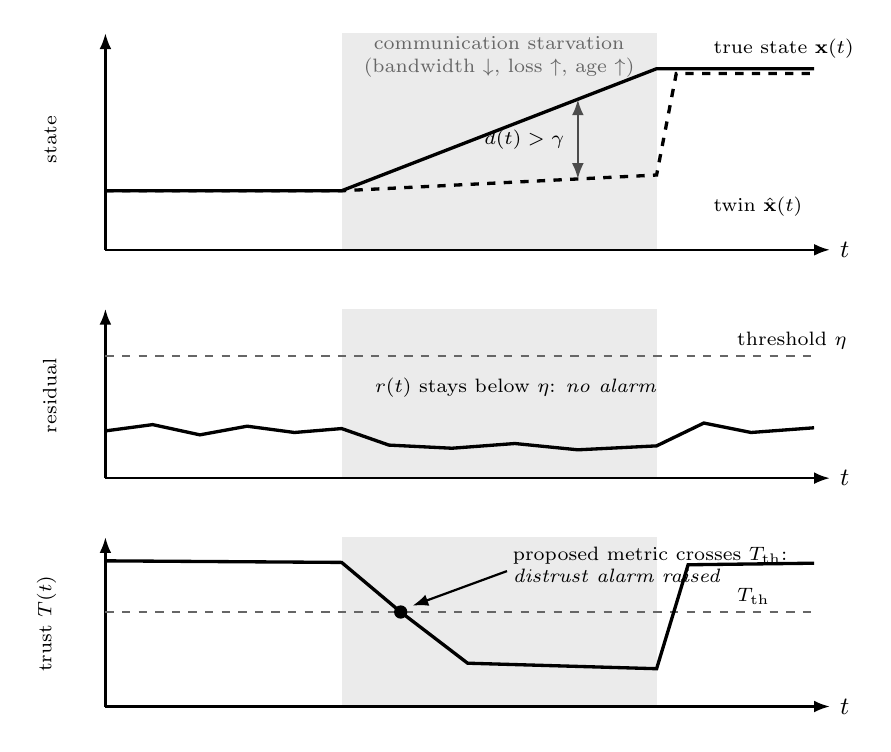
\begin{tikzpicture}[x=1cm,y=1cm,>={Latex[length=2mm]},font=\small]

%% ---------------- panel 1 : states -------------------------------
\begin{scope}[shift={(0,6.0)}]
  \fill[black!8] (3,0) rectangle (7,2.75);
  \node[align=center,font=\scriptsize,text=black!60] at (5,2.45)
      {communication starvation\\(bandwidth $\downarrow$, loss $\uparrow$, age $\uparrow$)};
  \draw[->,thick] (0,0) -- (9.2,0) node[right]{$t$};
  \draw[->,thick] (0,0) -- (0,2.75);
  \node[rotate=90,anchor=south,font=\scriptsize] at (-0.5,1.4) {state};
  % true state
  \draw[very thick] (0,0.75) -- (3,0.75) -- (7,2.30) -- (9.0,2.30);
  \node[anchor=west,font=\scriptsize] at (7.6,2.55) {true state $\bx(t)$};
  % twin estimate
  \draw[very thick,dashed] (0,0.75) -- (3,0.75) -- (7,0.95) -- (7.25,2.24) -- (9.0,2.24);
  \node[anchor=west,font=\scriptsize] at (7.6,0.55) {twin $\bxh(t)$};
  % divergence arrow
  \draw[<->,thick,black!70] (6,0.90) -- (6,1.91);
  \node[anchor=east,font=\scriptsize] at (5.95,1.40) {$d(t)>\gamma$};
\end{scope}

%% ---------------- panel 2 : residual -----------------------------
\begin{scope}[shift={(0,3.1)}]
  \fill[black!8] (3,0) rectangle (7,2.15);
  \draw[->,thick] (0,0) -- (9.2,0) node[right]{$t$};
  \draw[->,thick] (0,0) -- (0,2.15);
  \node[rotate=90,anchor=south,font=\scriptsize] at (-0.5,1.05) {residual};
  \draw[dashed,thick,black!60] (0,1.55) -- (9.0,1.55);
  \node[anchor=west,font=\scriptsize] at (7.9,1.75) {threshold $\eta$};
  \draw[very thick] (0,0.60) -- (0.6,0.68) -- (1.2,0.55) -- (1.8,0.66)
        -- (2.4,0.58) -- (3.0,0.63) -- (3.6,0.42) -- (4.4,0.38)
        -- (5.2,0.44) -- (6.0,0.36) -- (7.0,0.41) -- (7.6,0.70)
        -- (8.2,0.58) -- (9.0,0.64);
  \node[anchor=west,font=\scriptsize,align=left] at (3.3,1.15)
      {$r(t)$ stays below $\eta$: \emph{no alarm}};
\end{scope}

%% ---------------- panel 3 : trust --------------------------------
\begin{scope}[shift={(0,0.2)}]
  \fill[black!8] (3,0) rectangle (7,2.15);
  \draw[->,thick] (0,0) -- (9.2,0) node[right]{$t$};
  \draw[->,thick] (0,0) -- (0,2.15);
  \node[rotate=90,anchor=south,font=\scriptsize] at (-0.5,1.05) {trust $T(t)$};
  \draw[dashed,thick,black!60] (0,1.20) -- (9.0,1.20);
  \node[anchor=west,font=\scriptsize] at (7.9,1.40) {$T_{\mathrm{th}}$};
  \draw[very thick] (0,1.85) -- (3,1.83) -- (3.75,1.20) -- (4.6,0.55)
        -- (7,0.48) -- (7.4,1.80) -- (9.0,1.82);
  \fill (3.75,1.20) circle (2.4pt);
  \draw[->,thick] (5.1,1.72) -- (3.9,1.28);
  \node[anchor=west,font=\scriptsize,align=left] at (5.05,1.80)
      {proposed metric crosses $T_{\mathrm{th}}$:\\\emph{distrust alarm raised}};
\end{scope}

\end{tikzpicture}}
\caption{Silent drift: twin--grid divergence grows under communication
starvation while residual- and age-based detectors remain below their
alarm thresholds. Top: the true state moves while the starved twin
estimate stalls, so divergence $d(t)$ exceeds the operator tolerance
$\gamma$. Middle: because few fresh measurements arrive, the classical
residual $r(t)$ never approaches its threshold $\eta$---the ``silent''
part of the failure. Bottom: the proposed communication-aware trust
metric falls because the \emph{exposure} term responds to the scarcity
itself. Schematic; not experimental data.}
\label{fig:concept}
\end{figure*}

\subsection*{Contributions}
This paper makes the following contributions.
\begin{itemize}
\item We formalize \emph{silent drift} for a distribution-grid DT
operating over a constrained telemetry network, and define the
communication-state variables (bandwidth, latency/age, packet loss,
energy) that govern it (Section~\ref{sec:model}).
\item We define a \textbf{communication-aware trust metric} whose novel
component is an \emph{excess silent-drift exposure} term equal to the
additional state unobservability induced by finite communication relative
to perfect telemetry, combined with a received-measurement residual term
(Section~\ref{sec:metric}).
\item We establish structural properties of the metric, including a
\textbf{reduction property}: under unlimited telemetry the exposure term
vanishes and the metric collapses to a residual-consistency detector, so
the metric is a strict generalization of classical residual-based
detection rather than a distinct heuristic
(Section~\ref{sec:metric}, Propositions~\ref{prop:range}--\ref{prop:reduction}).
\item We \textbf{derive} the freshness discount from the state process
rather than assuming it, obtaining a hyperbolic law
$g_i(\Delta)=(1+\Delta/\tau_i)^{-1}$ with a per-channel time constant
$\tau_i=\sigma_i^{2}/\bh_i^{\top}\bQ\bh_i$ fixed by the process-noise
intensity, thereby eliminating a free tuning parameter
(Lemma~\ref{lem:age}).
\item We give a \textbf{$\delta$-confident exposure} that closes the
Jensen gap inherent in mean-information constructions, providing a
high-probability upper bound on realized posterior variance while
preserving the reduction property (Proposition~\ref{prop:confident}).
\item We prove that the \textbf{trivial communication-aware statistics are
cardinality-blind}, yielding an explicit AUC ceiling $1-q/2$ that
localizes the value of the information-geometric construction in
observability \emph{geometry} rather than channel count, and we design the
evaluation around that result (Proposition~\ref{prop:cardinality}).
\item We characterize the \textbf{exposure ceiling} induced by
regularization and derive a necessary condition on the regularization
level for the metric to be able to alarm at all under total starvation
(Proposition~\ref{prop:ceiling}).
\item We design an evaluation that pits the metric against classical
residual- and robust-estimator baselines \emph{and against trivial
communication-aware controls}, and we pre-register \textbf{three}
falsification criteria---covering the existence of the phenomenon,
separability from the classical baseline, and the necessity of the
information-geometric construction
(Sections~\ref{sec:setup}--\ref{sec:results}).
\end{itemize}

The remainder of the paper is organized as follows.
Section~\ref{sec:related} reviews DT trust, bad-data detection and robust
state estimation, age-based qualifiers, and communication-aware DTs,
stating the gap relative to each. Section~\ref{sec:model} presents the
system model and the definition of silent drift.
Section~\ref{sec:metric} defines the trust metric and its properties.
Section~\ref{sec:setup} describes the experimental setup, and
Section~\ref{sec:results} reports the completed information-geometry
diagnostics and, once the predeclared evidence gate is satisfied, the
confirmatory campaign results.
Section~\ref{sec:discussion} discusses separability, limitations, and
threats to validity, and Section~\ref{sec:conclusion} concludes.

% =====================================================================
\section{Related Work and Background}
\label{sec:related}

Fig.~\ref{fig:positioning} summarizes the positioning of this work along
two axes that matter for the contribution: whether a method makes
communication resources \emph{explicit arguments} of its trust or quality
signal, and whether it provides a \emph{trust-metric / detectability}
characterization as opposed to an estimator, scheduler, or filter.

\begin{figure}[!t]
\centering
\resizebox{0.96\columnwidth}{!}{%
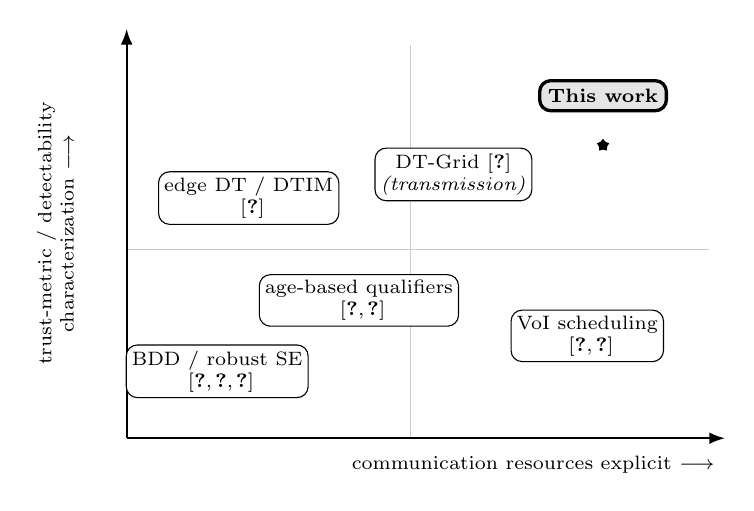
\begin{tikzpicture}[x=1cm,y=1cm,>={Latex[length=2mm]},font=\small]
  \draw[black!20] (0,2.4) -- (7.4,2.4);
  \draw[black!20] (3.6,0) -- (3.6,5.0);
  \draw[->,thick] (0,0) -- (7.6,0)
      node[below left=1mm and 0mm,font=\scriptsize,align=center]
      {communication resources explicit $\longrightarrow$};
  \draw[->,thick] (0,0) -- (0,5.2);
  \node[rotate=90,anchor=south,font=\scriptsize,align=center] at (-0.55,2.6)
      {trust-metric / detectability\\characterization $\longrightarrow$};

  \node[draw,rounded corners,fill=white,inner sep=2pt,font=\scriptsize,align=center]
      (bdd) at (1.15,0.85) {BDD / robust SE\\\cite{abur2004,handschin1975,gol2014lav}};
  \node[draw,rounded corners,fill=white,inner sep=2pt,font=\scriptsize,align=center]
      (age) at (2.95,1.75) {age-based qualifiers\\\cite{duran2023,cosandal2026}};
  \node[draw,rounded corners,fill=white,inner sep=2pt,font=\scriptsize,align=center]
      (edt) at (1.55,3.05) {edge DT / DTIM\\\cite{guo2025}};
  \node[draw,rounded corners,fill=white,inner sep=2pt,font=\scriptsize,align=center]
      (dtg) at (4.15,3.35) {DT-Grid \cite{dtgrid2026}\\\emph{(transmission)}};
  \node[draw,rounded corners,fill=white,inner sep=2pt,font=\scriptsize,align=center]
      (voi) at (5.85,1.30) {VoI scheduling\\\cite{bui2024,molin2019}};
  \node[draw,rounded corners,very thick,fill=black!10,inner sep=3pt,
        font=\scriptsize\bfseries,align=center]
      (ours) at (6.05,4.35) {This work};
  \node[star,star points=5,fill=black,inner sep=1.1pt] at (6.05,3.72) {};
\end{tikzpicture}}
\caption{Positioning relative to the closest identified prior art. The
proposed metric is communication-resource-explicit and
silent-drift-targeted for a distribution-grid DT. DT-Grid
\cite{dtgrid2026} is the nearest conceptual neighbour but is evaluated on
a transmission benchmark and its trust signal remains a residual with a
confidence envelope.}
\label{fig:positioning}
\end{figure}

\subsection{Digital-twin trust for power systems}
Trust and trustworthiness for digital twins have been framed at the
standards and taxonomy level---security and trust considerations for DT
technology~\cite{voas2023}, the general problem of ``trusting'' a
twin~\cite{laplante2022}, assurance frameworks for physical model-based
twins in other domains~\cite{jeon2024}, authentication of grid twins
against real-world anchors~\cite{hatami2025}, and recent taxonomies of
trustworthy twinning~\cite{trustworthy2025}. These works establish
\emph{that} trust must be quantified; they do not supply a
resource-parameterized metric for a distribution-grid twin.

DT-Grid~\cite{dtgrid2026} is the closest competitor to the present work.
It couples communication degradation to trust by allowing latency and
packet loss to inflate Huber-weighted robust state-estimation residuals
and by maintaining a confidence envelope that makes downstream dispatch
conservative when telemetry is degraded. Three distinctions are concrete
and central to this paper. First, DT-Grid's trust signal is a residual
(with a confidence envelope) and is therefore subject to the silent-drift
failure mode---when starvation suppresses residuals, the envelope need not
widen for the right reason. Second, bandwidth, loss, and age are not arguments of DT-Grid's trust
value. We claim a resource-parameterized \emph{metric}; we do \emph{not}
claim a resource-parameterized \emph{characterization of detectability}
(a bound of the form $P_D\ge f(b,\Delta,p)$), which neither DT-Grid nor
this paper provides and which we identify as open in
Section~\ref{sec:discussion}-D. Third, its evaluation
is on a transmission benchmark rather than an unbalanced distribution
feeder, so it is a \emph{conceptual} nearest neighbour rather than a
like-for-like distribution-grid competitor. Our metric instead makes
communication resources explicit arguments of the trust value and adds an
exposure term that grows precisely when telemetry is starved, independent
of the instantaneous residual. We do not claim DT-Grid is incorrect; we
claim it lacks a communication-parameterized trust metric and does not
target silent drift.

\subsection{Bad-data detection and robust state estimation}
Classical bad-data detection---largest-normalized-residual and chi-square
tests~\cite{abur2004,handschin1975}, with comparative
studies~\cite{mili1985} and methods for multiple interacting bad
data~\cite{cheniae1996}---and robust estimators such as Huber and
LAV~\cite{gol2014lav,gol2014three,monticelli1999,wang2017robust} are the
standard tools for identifying untrustworthy measurements. In the
distribution setting the estimation problem is additionally unbalanced and
weakly observable~\cite{baran1994,singh2009}, which sharpens rather than
softens the issue. A closely related literature detects deliberately
falsified measurements---false data injection attacks and their
detection~\cite{liu2011,kosut2011,liang2017,chaojun2015,he2017}. All of
these methods are powerful when measurements are present but corrupted.
They are, by design, evidence-driven: their detection statistic is a
function of received residuals. The gap we fill is the regime where the
\emph{absence or staleness} of measurements, rather than their corruption,
drives divergence; there, residual statistics are uninformative, and a low
residual under starvation is not evidence of trust. Our metric is
constructed to reduce to a residual detector in the unlimited-telemetry
limit (Section~\ref{sec:metric}) and to depart from it exactly when
communication is constrained.

\subsection{Age-based qualifiers}
The Age of Twin~\cite{duran2023} and Age of Staleness~\cite{cosandal2026}
quantify the freshness (and, for~\cite{cosandal2026}, the semantic
relevance) of the twin's information, drawing on the AoI
literature~\cite{kaul2012,kosta2017,yates2021} and its variants such as
the Age of Incorrect Information~\cite{maatouk2020}. These are important
precursors but are not resource-parameterized trust metrics for grids: age
measures elapsed time since update but does not, on its own, bound how
much undetected state divergence that age permits, nor does it fuse with
measurement evidence. Our exposure term can be viewed as translating age,
loss, and bandwidth scarcity---through the measurement model---into a
bound on undetected divergence, which is then combined with residual
evidence.

\subsection{Communication-aware DTs and sensing/communication scheduling}
Digital twins of and over wireless systems are surveyed
in~\cite{khan2022,mihai2022}, with model-driven Bayesian approaches to
joint optimization and monitoring~\cite{ruah2023} and recent work on
deployment and synchronization in twin-empowered
networks~\cite{farag2026}. Value-of-Information (VoI) sensor scheduling
for cloud-based DTs~\cite{bui2024} shows that communication overhead can
be reduced substantially while maintaining a DT-accuracy target, building
on a broader VoI and sensor-scheduling
literature~\cite{soleymani2022,molin2019,chiariotti2022,shi2011}; but it
addresses generic networked control rather than distribution grids and
concerns \emph{scheduling} rather than a \emph{trust metric}. The Edge
Digital Twin of~\cite{guo2025} includes a Data Trustworthiness
Identification Module that thresholds a normalized command-deviation
quantity and substitutes a twin-deduced setpoint; this is a bad-data /
false-data-injection-style filter with no communication-parameterized
metric and no resource characterization. The estimation-theoretic
consequences of lossy links are classical~\cite{sinopoli2004,schenato2007}
and motivate our use of an information-matrix construction rather than a
residual one. Reference~\cite{bui2024} is context for a later paper in
this thesis and is not a competitor to the metric defined here.

\subsection{Gap statement}
No published work defines, for a distribution-grid DT, a trust metric that
(i) is an explicit function of bandwidth, latency, packet loss, and energy
and (ii) is designed to detect silent drift that residual- and age-based
methods miss. This paper provides such a metric and tests it against the
strongest available baselines, including a no-communication-limit oracle.

% =====================================================================
\section{System Model}
\label{sec:model}

Table~\ref{tab:notation} collects the notation used throughout.
Fig.~\ref{fig:architecture} shows the corresponding signal path.

\begin{table}[!t]
\caption{Notation.}
\label{tab:notation}
\centering
\footnotesize
\renewcommand{\arraystretch}{1.15}
\begin{tabular}{@{}l p{5.6cm}@{}}
\toprule
Symbol & Meaning (units; per-unit unless stated) \\
\midrule
$\mathcal{B}$, $N$ & bus set of the feeder; $N=|\mathcal{B}|$ \\
$\bx(t)\in\mathbb{R}^{n}$ & true physical grid state at time $t$ \\
$\bW_{\!\mathrm{est}}$ & age-aware estimator weights $g_i\sigma_i^{-2}$, Eq.~\eqref{eq:estimator} \\
$\bxh(t)\in\mathbb{R}^{n}$ & twin's state estimate \\
$n$ & state dimension; $n=491$ in the implemented supernode-coordinate model \\
$\mathcal{M}$, $m$ & measurement set; $m=|\mathcal{M}|$ \\
$z_i$ & value of measurement $i$ \\
$\bh_i^{\top}$ & $i$-th row of the measurement Jacobian $\bH$ \\
$\sigma_i^{2}$ & noise variance of measurement $i$ \\
$\Mrx(t)$ & channels whose latest sample is received and current \\
$b_i$, $b_i^{\min}$ & allocated / minimum required bandwidth (bit/s) \\
$\Delta_i(t)$ & age of channel $i$ (s) \\
$p_i$ & packet-loss probability of channel $i$ \\
$\varepsilon_i$, $E$ & energy per report; per-node energy budget (J) \\
$\bc(t)$ & aggregate communication state $\{(b_i,\Delta_i,p_i,\varepsilon_i)\}$ \\
$\rho_i(t)\in[0,1]$ & effective channel reliability \\
$g_i(\cdot)$, $\tau_i$ & derived freshness discount and its per-channel
time constant (s), Lemma~\ref{lem:age} \\
$\bQ$ & process-noise intensity (per unit time) \\
$\delta$, $s_\delta$ & confidence level and Bernstein deflation, Prop.~\ref{prop:confident} \\
$\bar V,\bar L,\phi$ & monotone deflation envelopes, Eq.~\eqref{eq:envelopes} \\
$k_\delta$, $\Lambda_k$ & loss quantile and top-$k$ norm sum, Eq.~\eqref{eq:quantfloor} \\
$J(\bxh)$ & weighted residual sum of squares ($\chi^{2}$ statistic) \\
$q$ & fraction of cardinality-matched event pairs, Prop.~\ref{prop:cardinality} \\
$\bG(t)$, $\bG_{\infty}$ & communication-weighted / perfect-telemetry information matrix \\
$\epsilon$ & information-matrix regularization level \\
$\omega$ & per-update state-increment bound (drift-rate bound) \\
$u(t)$ & excess silent-drift exposure \\
$r(t)$ & age-consistent received-measurement residual, Eq.~\eqref{eq:residual} \\
$r_0,u_0$ & normalizing constants for $r$ and $u$ \\
$T(t)\in(0,1]$ & trust metric; alarm when $T(t)<T_{\mathrm{th}}$ \\
$s(t)$ & equivalent distrust statistic $r/r_0+u/u_0$ \\
$d(t)$ & twin--grid divergence $\lVert\bx-\bxh\rVert_{\bW}$ \\
$\bW\succ0$ & divergence weighting matrix \\
$\gamma$ & operator divergence tolerance \\
$\eta$ & classical residual-detector threshold \\
\bottomrule
\end{tabular}
\end{table}

\subsection{Grid and digital twin}
Let the feeder have bus set $\mathcal{B}$ with $|\mathcal{B}|=N$. The
physical grid state at time $t$ is $\bx(t)\in\mathbb{R}^{n}$. In the
implemented feeder model, $n=491$ and the state stacks 244 non-slack
supernode voltage angles with 247 supernode voltage magnitudes, expressed
in radians and per unit. The digital twin maintains an
estimate $\bxh(t)$ produced by an \textbf{age-aware} weighted-least-squares
(or robust) estimator over the measurements received by time
$t$~\cite{abur2004,monticelli1999}, with the three-phase unbalanced
formulation appropriate to distribution~\cite{baran1994,singh2009}. By
``age-aware'' we mean that the estimator weights channel $i$ by the inverse
of the \emph{effective} variance of Lemma~\ref{lem:age},
\begin{equation}
\bxh(t)=\arg\min_{\bx}\sum_{i\in\Mrx(t)}
\frac{g_i(\Delta_i(t))}{\sigma_i^{2}}\big(z_i-\bh_i^{\top}\bx\big)^{2},
\label{eq:estimator}
\end{equation}
rather than by $\sigma_i^{-2}$. This is not a stylistic preference: it is
required for the internal consistency of the metric, as
Remark~\ref{rem:estcoupling} shows. For the Huber and LAV comparison
arms, the same effective weights enter the robust objective. All
quantities are expressed in per unit so that state, measurement, and
information quantities are dimensionally commensurate
(Remark~\ref{rem:units}).

\subsection{Measurements}
Let $\mathcal{M}$ be the measurement set, $|\mathcal{M}|=m$. Measurement
$i\in\mathcal{M}$ has value $z_i$, measurement-function Jacobian row
$\bh_i^{\top}$ (the $i$-th row of $\bH$), and noise variance
$\sigma_i^{2}$. The experiment uses additive zero-mean Gaussian noise
with variances frozen in the feeder artifact; all detector arms receive
the same noisy realization within a paired cell.

\subsection{Constrained communication network}
Telemetry from field devices to the twin traverses a communication network
with finite resources. For each measurement channel $i$ we define the
communication-state variables:
\begin{itemize}
\item allocated bandwidth $b_i$ (bit/s), with per-channel minimum
$b_i^{\min}$ required to deliver one report within the sampling period;
\item age $\Delta_i(t)\ge0$, the elapsed time since the twin last received
a fresh sample on channel $i$ (this captures latency, jitter, and
under-sampling jointly)~\cite{kaul2012,yates2021};
\item packet-loss probability $p_i\in[0,1]$;
\item energy per report $\varepsilon_i$ and a per-node energy budget $E$,
which constrain the feasible sampling/transmission rate (and hence can
inflate $\Delta_i$ through duty-cycling)~\cite{shi2011}. Energy is treated
as an indirect feasibility constraint in Paper~1 rather than as a
separately swept factor.
\end{itemize}
Let $\Mrx(t)\subseteq\mathcal{M}$ denote the subset of channels whose most
recent sample has been received and is current at time $t$. The aggregate
communication state is
$\bc(t)=\{(b_i,\Delta_i(t),p_i,\varepsilon_i)\}_{i\in\mathcal{M}}$.

\begin{figure*}[!t]
\centering
\resizebox{0.97\textwidth}{!}{%
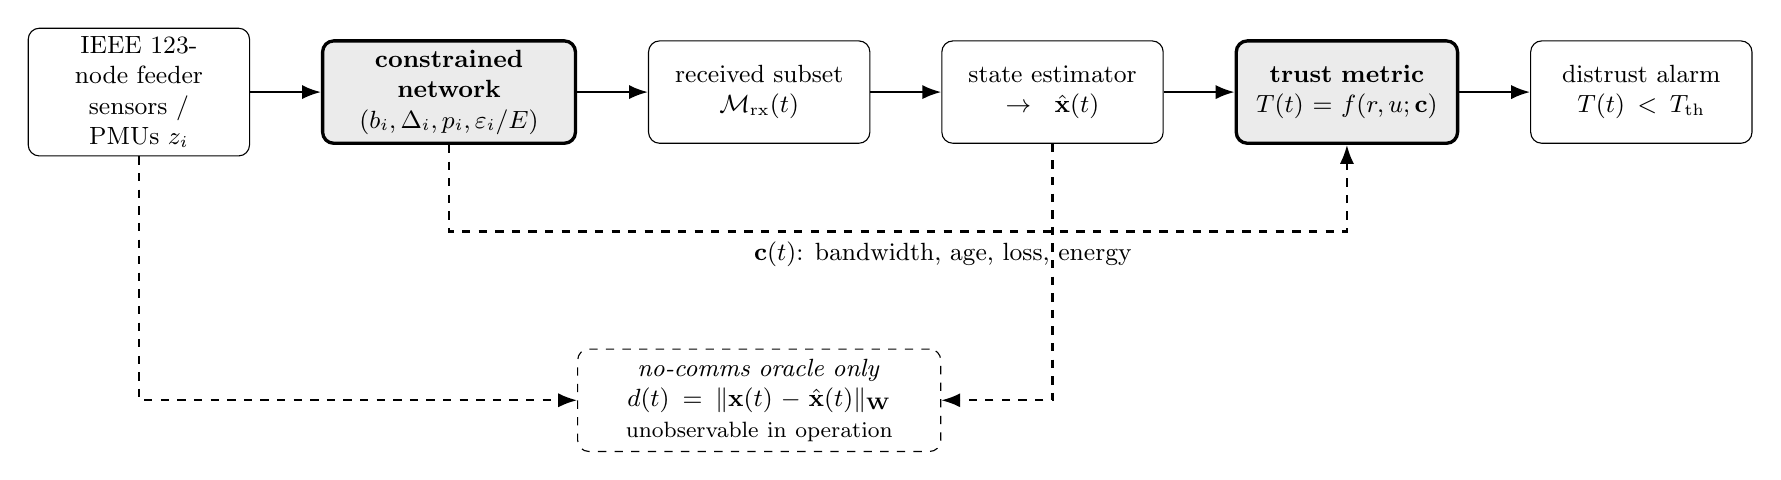
\begin{tikzpicture}[
  >={Latex[length=2.4mm]},
  box/.style={draw,rounded corners,align=center,font=\small,
              minimum height=13mm,text width=26mm,inner sep=3pt,fill=white},
  net/.style={draw,very thick,rounded corners,align=center,font=\small,
              minimum height=13mm,text width=30mm,inner sep=3pt,fill=black!8},
  trust/.style={draw,very thick,rounded corners,align=center,font=\small,
              minimum height=13mm,text width=26mm,inner sep=3pt,fill=black!8}]

\node[box]                        (grid)  at (0,0)
   {IEEE 123-node feeder\\sensors / PMUs $z_i$};
\node[net, right=9mm of grid]     (net)
   {\textbf{constrained network}\\$(b_i,\Delta_i,p_i,\varepsilon_i/E)$};
\node[box, right=9mm of net]      (rx)
   {received subset\\$\Mrx(t)$};
\node[box, right=9mm of rx]       (se)
   {state estimator\\$\rightarrow\ \bxh(t)$};
\node[trust, right=9mm of se]     (trust)
   {\textbf{trust metric}\\$T(t)=f(r,u;\bc)$};
\node[box, right=9mm of trust]    (alarm)
   {distrust alarm\\$T(t)<T_{\mathrm{th}}$};

\draw[->,thick] (grid)  -- (net);
\draw[->,thick] (net)   -- (rx);
\draw[->,thick] (rx)    -- (se);
\draw[->,thick] (se)    -- (trust);
\draw[->,thick] (trust) -- (alarm);

% communication state feeds the trust metric directly
\draw[->,thick,dashed] (net.south) -- ++(0,-11mm)
      -- node[below,font=\small,pos=0.55] {$\bc(t)$: bandwidth, age, loss, energy}
      ($(trust.south)+(0,-11mm)$) -- (trust.south);

% oracle
\node[box,dashed,below=26mm of rx,text width=44mm] (oracle)
   {\emph{no-comms oracle only}\\
    $d(t)=\lVert\bx(t)-\bxh(t)\rVert_{\bW}$\\
    {\footnotesize unobservable in operation}};
\draw[->,thick,dashed] (grid.south) |- (oracle.west);
\draw[->,thick,dashed] (se.south)   |- (oracle.east);
\end{tikzpicture}}
\caption{System model: telemetry from the feeder traverses a bandwidth-,
latency-, loss-, and energy-constrained network before reaching the twin's
estimator. The communication state $\bc(t)$ is an explicit input to the
trust metric (dashed), which is what distinguishes it from residual-only
signals. The true divergence $d(t)$ is unobservable in operation and is
available only to the no-communication-limit oracle.}
\label{fig:architecture}
\end{figure*}

\subsection{Divergence and the definition of silent drift}
Define the twin--grid divergence
\begin{equation}
d(t)\;=\;\lVert \bx(t)-\bxh(t)\rVert_{\bW},
\label{eq:divergence}
\end{equation}
where $\bW\succ0$ is the frozen divergence weighting matrix. The
experiment uses the predeclared identity matrix, $\bW=\bI_{491}$, so the
oracle label is not tailored to the information geometry of the proposed
metric. Note that $d(t)$ is computable only when the true state
$\bx(t)$ is known; in operation it is unobservable, and in this study it
is available only to the no-communication-limit oracle
(Section~\ref{sec:setup}). Let $\gamma>0$ be an operator-defined
divergence tolerance and let $\eta$ be the detection threshold of a
classical residual detector; proposed calibration ranges for both are
given in Table~\ref{tab:hyper}.

\begin{definition}[Drift event]
\label{def:driftevent}
A \emph{drift event} on interval $[t_0,t_1]$ is a period during which the
true divergence exceeds the operator tolerance, $d(t)>\gamma$, under a
stated communication regime. Drift events are labelled by the oracle from
the ground-truth state and are the positive class throughout
Section~\ref{sec:results}.
\end{definition}

\begin{definition}[Residual-silent event; silence rate]
\label{def:silentdrift}
A drift event is \emph{residual-silent} if, throughout $[t_0,t_1]$, the
classical residual detector applied to the received measurements does not
alarm (its statistic stays below $\eta$). The \emph{silence rate}
$S(\text{regime})$ is the fraction of drift events in a given
communication regime that are residual-silent. \emph{Silent drift} is the
phenomenon of residual-silent drift events occurring at non-negligible
rate under communication starvation.
\end{definition}

\begin{remark}[Why the label must not reference the baseline]
\label{rem:circularity}
An earlier formulation of this work folded the residual-silence condition
into the \emph{definition} of the positive class. That is circular: if
positives are defined to satisfy ``the residual detector does not alarm,''
then the residual detector's statistic is bounded below $\eta$ on every
positive by construction, its true-positive rate is zero by construction,
and any method responding to anything other than the residual outperforms
it \emph{a priori}. No experiment could then falsify the paper's claim.
Definitions~\ref{def:driftevent}--\ref{def:silentdrift} separate the two
roles: the positive class is defined \emph{only} by ground-truth
divergence, and residual-silence becomes a \emph{measured} property. The
silence rate $S$ is consequently a primary empirical result of this paper
rather than an assumption: if $S\approx0$ even
under severe starvation, then silent drift is not an operationally
significant phenomenon and the motivation for the metric collapses. We
regard this as the paper's first falsification opportunity.
\end{remark}

The objective of Section~\ref{sec:metric} is a trust metric that
decreases during drift events even when those events are residual-silent.
Whether it does so, and whether it does so better than both classical and
\emph{trivial} communication-aware statistics, is the empirical question
of Sections~\ref{sec:setup}--\ref{sec:results}.

% =====================================================================
\section{The Communication-Aware Trust Metric}
\label{sec:metric}

We construct a trust value $T(t)\in(0,1]$ (higher is more trustworthy)
from two ingredients: a \textbf{received-measurement residual term}
$r(t)$, which captures divergence that \emph{does} manifest in the
telemetry, and an \textbf{excess silent-drift exposure term} $u(t)$, which
captures divergence that \emph{could} accumulate undetected given the
current communication state. The exposure term is the
communication-aware core of the metric. Fig.~\ref{fig:blockdiagram} shows
the construction.

\subsection{Effective channel reliability, with a derived freshness discount}
Earlier versions of this construction posited an exponential freshness
discount $g(\Delta)=e^{-\Delta/\tau}$ with a free global time constant
$\tau$. That form is not necessary: the information that a \emph{stale}
measurement carries about the \emph{current} state follows from the state
dynamics, and is derived below.

\begin{assumption}[State process]
\label{as:process}
Between updates the state follows a driftless Gauss--Markov (random-walk)
process $d\bx=\bQ^{1/2}d\mathbf{W}$ with process-noise intensity
$\bQ\succeq0$ per unit time, independent of the measurement noise. The
experiment uses the $\bQ$ matrix estimated and frozen with the feeder
artifact before the evaluation seeds are generated.
\end{assumption}

\begin{lemma}[Information content of an aged measurement]
\label{lem:age}
Under Assumption~\ref{as:process}, a measurement of channel $i$ taken at
time $t-\Delta_i$ contributes to the information about $\bx(t)$ exactly
\begin{equation}
\frac{\bh_i\bh_i^{\top}}{\sigma_i^{2}+\Delta_i\,\bh_i^{\top}\bQ\bh_i}
\;=\;g_i(\Delta_i)\,\sigma_i^{-2}\bh_i\bh_i^{\top},
\label{eq:agedinfo}
\end{equation}
where the freshness discount and its time constant are
\begin{equation}
\boxed{\;g_i(\Delta)=\Big(1+\frac{\Delta}{\tau_i}\Big)^{-1},
\qquad
\tau_i=\frac{\sigma_i^{2}}{\bh_i^{\top}\bQ\bh_i}.\;}
\label{eq:gderived}
\end{equation}
\end{lemma}
\begin{IEEEproof}
Write $\bx(t-\Delta_i)=\bx(t)-\mathbf{w}_i$ with
$\mathbf{w}_i=\bx(t)-\bx(t-\Delta_i)$, so that
$\mathbf{w}_i\sim\mathcal{N}(\mathbf{0},\bQ\Delta_i)$ by
Assumption~\ref{as:process}. The measurement equation
$z_i=\bh_i^{\top}\bx(t-\Delta_i)+v_i$ becomes
$z_i=\bh_i^{\top}\bx(t)+\tilde v_i$ with
$\tilde v_i=v_i-\bh_i^{\top}\mathbf{w}_i$. Since $v_i$ and
$\mathbf{w}_i$ are independent,
$\operatorname{Var}(\tilde v_i)=\sigma_i^{2}+\Delta_i\bh_i^{\top}\bQ\bh_i$.
Regarded as a measurement of $\bx(t)$, channel $i$ therefore has effective
variance $\sigma_i^2+\Delta_i\bh_i^\top\bQ\bh_i$ and contributes the
Fisher information \eqref{eq:agedinfo}; factoring out $\sigma_i^{-2}$
gives \eqref{eq:gderived}.
\end{IEEEproof}

The effective reliability is then
\begin{equation}
\rho_i(t)\;=\;(1-p_i)\,g_i\!\big(\Delta_i(t)\big)\,
\mathbf{1}\!\big[b_i\ge b_i^{\min}\big],\qquad \rho_i(t)\in[0,1],
\label{eq:rho}
\end{equation}
with $g_i$ now \emph{derived} rather than assumed. Energy enters through
the feasible set for $(b_i,\text{sampling rate})$ and hence through
$\Delta_i$~\cite{shi2011}; energy is not independently manipulated in
the present factorial campaign.

\begin{remark}[Hyperbolic, not exponential --- and why the difference
matters precisely in the regime of interest]
\label{rem:hyperbolic}
Three consequences follow from Lemma~\ref{lem:age}.
\emph{(i) The free constant is eliminated.} $\tau_i$ is no longer a tuning
parameter but a per-channel physical quantity---the age at which
process-noise uncertainty along $\bh_i$ equals the measurement noise
variance. It is determined by $\bQ$, which is identifiable from load
dynamics, and it differs across channels, whereas the earlier $\tau$ was
one number for the whole feeder.
\emph{(ii) The two forms agree only for fresh data.} Both satisfy
$g(0)=1$ and $g(x)=1-x+O(x^{2})$ for $x=\Delta/\tau$, which is why the
exponential appeared adequate. They diverge sharply for $\Delta\gtrsim\tau$:
at $\Delta/\tau=3$ the exponential returns $e^{-3}\approx0.050$ against
$1/4=0.25$, and at $\Delta/\tau=5$, $\approx0.0067$ against
$1/6\approx0.167$.
\emph{(iii) The direction of the error is unfavourable.} Since
$e^{-x}<(1+x)^{-1}$ for $x>0$, the exponential \emph{over}-penalizes stale
data, understating $\bG(t)$ and hence \emph{overstating} exposure at large
age. It is therefore conservative for detection but miscalibrated, and the
error is largest exactly under severe starvation.
\end{remark}

\begin{remark}[Exact multi-channel form]
\label{rem:exactage}
Equation \eqref{eq:gderived} treats channels independently. When several
channels are simultaneously stale their effective noises share process
noise: for a common driving Brownian motion,
$\operatorname{Cov}(\bh_i^{\top}\mathbf{w}_i,\bh_j^{\top}\mathbf{w}_j)
=\bh_i^{\top}\bQ\bh_j\min(\Delta_i,\Delta_j)$. The exact effective noise
covariance is therefore $\bSigma_{\mathrm{eff}}=\bR+\bPsi$ with
$\bPsi_{ij}=\bh_i^{\top}\bQ\bh_j\min(\Delta_i,\Delta_j)$, giving
$\bG_{\mathrm{exact}}=\bH^{\top}\bSigma_{\mathrm{eff}}^{-1}\bH$. Note
$\bPsi\succeq0$ by construction, being a covariance. Equation
\eqref{eq:rho} is the diagonal approximation
$\bPsi\approx\operatorname{diag}(\bPsi)$, exact when at most one channel
is stale. We use the diagonal form as the primary definition for
computational reasons and report $\bG_{\mathrm{exact}}$ as a cross-check
in the sensitivity analysis (Table~\ref{tab:sensitivity}).
\end{remark}

\subsection{Communication-weighted information and excess exposure}
Define the communication-weighted information matrix and the full
(perfect-telemetry) information matrix
\begin{equation}
\bG(t)=\!\sum_{i\in\mathcal{M}}\!\rho_i(t)\,\sigma_i^{-2}\bh_i\bh_i^{\top},
\qquad
\bG_{\infty}=\!\sum_{i\in\mathcal{M}}\!\sigma_i^{-2}\bh_i\bh_i^{\top}.
\label{eq:information}
\end{equation}
Here $\bG_{\infty}$ is the information available if every channel were
fresh, loss-free, and adequately provisioned ($\rho_i\equiv1$); it is the
classical Fisher information of the measurement
set~\cite{monticelli1985,wang2018crb}. We work throughout with the
\emph{regularized} inverse
\begin{equation}
\bG_{\epsilon}(t)\;=\;\big(\bG(t)+\epsilon\bI\big)^{-1},
\qquad \epsilon>0,
\label{eq:regularized}
\end{equation}
for reasons made precise in Remark~\ref{rem:pinv}. Assuming a bound
$\omega$ on the state increment between consecutive twin updates (a
ramp/Lipschitz bound on grid dynamics), fixed at $0.02$~p.u. per update,
define the \textbf{excess silent-drift exposure}
\begin{equation}
\boxed{\;
u(t)\;=\;\omega^{2}\,\nu\,
\Big(\lmax\!\big(\bG_{\epsilon}(t)\big)
     -\lmax\!\big((\bG_{\infty}+\epsilon\bI)^{-1}\big)\Big)_{\!+}\;}
\label{eq:exposure}
\end{equation}
where $(\cdot)_{+}=\max(\cdot,0)$, $\lmax$ is the largest eigenvalue, and
\begin{equation}
\nu \;=\; \Big[\lmax\!\big((\bG_{\infty}+\epsilon\bI)^{-1}\big)\Big]^{-1}
\label{eq:nu}
\end{equation}
is a normalizing constant; its dimensional role is given in
Remark~\ref{rem:units}.
Intuitively, $\lmax(\bG_{\epsilon}(t))$ is the worst-direction posterior
variance achievable under the current communication state; subtracting the
perfect-telemetry floor isolates the \emph{additional} unobservability
caused by finite communication; $\nu$ renders that excess a dimensionless
\emph{relative} quantity; and scaling by $\omega^{2}$ converts it into a
bound on the undetected divergence that drift can produce. An alternative
scalarization (e.g., $\operatorname{tr}(\bG_{\epsilon}(t))$ in place of
$\lmax$) is possible. We predeclare $\lmax$ as primary and trace as a
sensitivity analysis.

\begin{remark}[Why the regularized inverse is necessary, not merely convenient]
\label{rem:pinv}
The draft construction used the Moore--Penrose pseudo-inverse
$\bG(t)^{+}$. This is unsafe in exactly the regime the paper targets. If
starvation drives a direction of the state into unobservability, the
corresponding eigenvalue of $\bG(t)$ goes to zero and the pseudo-inverse
sets the associated inverse eigenvalue to zero rather than to
$+\infty$---so $\lmax(\bG(t)^{+})$ can \emph{decrease} under severe
starvation, and the exposure term would paradoxically report improved
trust at the moment the twin is least observable. The regularized inverse
\eqref{eq:regularized} removes the pathology: as $\bG(t)\to\mathbf{0}$,
$\bG_{\epsilon}(t)\to\epsilon^{-1}\bI$ and $\lmax\to\epsilon^{-1}$, its
maximum. It also makes Proposition~\ref{prop:commmono} unconditional. We
therefore adopt \eqref{eq:regularized} as the primary definition and treat
the pseudo-inverse form as a limiting case valid only while
$\operatorname{range}(\bG(t))=\operatorname{range}(\bG_{\infty})$.
\end{remark}

\begin{remark}[The mean-information exposure is optimistic under random loss]
\label{rem:jensen}
Let $a_i\sim\mathrm{Bernoulli}(1-p_i)$ be the arrival indicator, so the
\emph{realized} information is
$\bG_{\mathrm{real}}=\sum_i a_i\sigma_i^{-2}\bh_i\bh_i^{\top}$ and
$\mathbb{E}[\bG_{\mathrm{real}}]$ is exactly the $(1-p_i)$-weighted matrix
of \eqref{eq:information}. The $(1-p_i)$ factor in \eqref{eq:rho} is
therefore \emph{expected Fisher information}, not a heuristic. However,
\eqref{eq:exposure} evaluates
$(\mathbb{E}[\bG_{\mathrm{real}}]+\epsilon\bI)^{-1}$, whereas the
operationally relevant quantity is the expected posterior covariance
$\mathbb{E}[(\bG_{\mathrm{real}}+\epsilon\bI)^{-1}]$. Matrix inversion is
operator-convex on the positive-definite cone, so by Jensen's inequality
\begin{equation}
\mathbb{E}\big[(\bG_{\mathrm{real}}+\epsilon\bI)^{-1}\big]\;\succeq\;
\big(\mathbb{E}[\bG_{\mathrm{real}}]+\epsilon\bI\big)^{-1}.
\label{eq:jensen}
\end{equation}
Hence $u(t)$ \emph{systematically understates} the true expected exposure,
and the gap widens with the variance of the arrival process---that is,
precisely in the high-loss regime the metric targets. The construction is
thus conservative in the wrong direction. We report this as a known
limitation of the \emph{mean-information} form
\eqref{eq:exposure}. Proposition~\ref{prop:confident} below supplies a
remedy, though a precise one: it bounds a \emph{high-probability quantile
of the realized} worst-direction variance, which is the operationally
relevant object, rather than the \emph{expectation} appearing in
\eqref{eq:jensen}. These are distinct targets---a quantile bound does not
in general dominate an expectation---so we do not claim
Proposition~\ref{prop:confident} bounds
$\mathbb{E}[(\bG_{\mathrm{real}}+\epsilon\bI)^{-1}]$. In numerical
checks on redundant measurement sets $u^{\delta}$ exceeded both the mean
form and the realized expectation across all loss levels tested, dipping
below the mean form only by a relative amount of order $\max_ip_i$ in the
regime $\sum_ip_i\ll\delta$, where no channel is expected to be lost.
\end{remark}

\begin{remark}[$\lmax$ is agnostic to the direction drift actually takes]
\label{rem:direction}
The scalarization $\lmax(\bG_{\epsilon})$ reports the \emph{worst}
direction of unobservability, but drift occurs in whatever direction the
physical disturbance pushes. If a direction is poorly observed while
nothing is moving along it, $u(t)$ is large and the metric alarms in the
absence of drift. This---not residual noise---is the dominant
false-alarm mechanism of the proposed detector, and it predicts that
$T(t)$ will be conservative on feeders with a persistently weak
observability direction. A disturbance-weighted alternative, e.g.
$\lmax(\bSigma_{w}^{1/2}\bG_{\epsilon}\bSigma_{w}^{1/2})$ with
$\bSigma_{w}$ the drift covariance, or the softer
$\operatorname{tr}(\bG_{\epsilon})$, would trade worst-case conservatism
for calibration. All three scalarizations are swept in the sensitivity
analysis (Table~\ref{tab:sensitivity}).
\end{remark}

\begin{remark}[Self-reference in the Jacobian]
\label{rem:jacobian}
In the nonlinear AC problem the rows $\bh_i$ are evaluated at the current
operating point, which in operation is the \emph{twin's estimate}
$\bxh(t)$ --- itself possibly drifted. The exposure term therefore assesses
observability using a linearization whose validity degrades exactly when
divergence is large. We quantify this by recomputing $u(t)$ at the oracle's
true state offline and reporting the discrepancy
(Table~\ref{tab:sensitivity}); we do not claim the effect is negligible.
\end{remark}

\begin{remark}[The positive part in \eqref{eq:exposure} never binds]
\label{rem:posvacuous}
Since $\rho_i(t)\in[0,1]$ we have $\bG(t)\preceq\bG_{\infty}$, hence
$(\bG(t)+\epsilon\bI)^{-1}\succeq(\bG_{\infty}+\epsilon\bI)^{-1}$ and
$\lmax(\bG_{\epsilon}(t))\ge\lmax((\bG_{\infty}+\epsilon\bI)^{-1})$ for
every $t$. The operator $(\cdot)_{+}$ in \eqref{eq:exposure} is therefore
never active and is retained only for definiteness: $u(t)\ge0$ holds
structurally, not by clipping. The same is \emph{not} true of the
$\delta$-confident variant, where the floors in \eqref{eq:combfloor} are
genuinely clipped.
\end{remark}

\begin{remark}[Dimensional consistency and the role of $\nu$]
\label{rem:units}
With all quantities in per unit, $\bG$ carries units of inverse
state-squared and $\lmax(\bG_{\epsilon})$ units of state-squared. The
draft's difference form $\omega^{2}(\lmax(\bG^{+})-\lmax(\bG_{\infty}^{-1}))$
therefore multiplies two state-squared quantities and is not commensurate
with $d^{2}$ as defined in~\eqref{eq:divergence}. Introducing $\nu$
in~\eqref{eq:nu} makes the bracketed excess a dimensionless relative
quantity, so $u(t)$ carries the units of $\omega^{2}$ and is directly
comparable with $d^{2}$ and $\gamma^{2}$. It additionally makes $u$
invariant to a common rescaling of all measurement variances, which is
desirable when comparing scenarios. Note that $\nu$ is \emph{not}
separately identifiable from $u_0$ when $\bG_{\infty}$ is fixed across all
scenarios---the two collapse into one constant---but it does matter when
the measurement set or topology varies across scenarios, which is the case
in our topology-change drift events. We therefore retain it explicitly;
equivalently, \eqref{eq:exposure} is the ratio form
$\omega^{2}[\lmax(\bG_{\epsilon})/\lmax((\bG_{\infty}+\epsilon\bI)^{-1})-1]_{+}$.
\end{remark}

\subsection{Received-measurement residual}
Let the age-consistent received-measurement residual (variance-normalized
innovation squared, corrected for staleness per Lemma~\ref{lem:age}) be
\begin{equation}
r(t)\;=\;\frac{1}{m}
\sum_{i\in\Mrx(t)}
g_i\!\big(\Delta_i(t)\big)\,
\frac{\big(z_i-\bh_i^{\top}\bxh(t)\big)^{2}}{\sigma_i^{2}},
\label{eq:residual}
\end{equation}
where $m=|\mathcal{M}|$ is the \emph{total} channel count and
$g_i(\cdot)$ is the \emph{same} freshness discount derived in
Lemma~\ref{lem:age}. The weight $g_i$ is not a heuristic down-weighting of
stale data: it is exactly the variance correction required for
consistency with Lemma~\ref{lem:age}, as Remark~\ref{rem:ageconsistent}
explains. At zero age $g_i=1$ and \eqref{eq:residual} is the classical
weighted residual sum of squares---the statistic of the $\chi^{2}$
bad-data test~\cite{abur2004,handschin1975}---divided by $m$. When $\Mrx(t)=\varnothing$ the sum is empty and $r(t)=0$ as a
continuous limit, not as a special convention. This term is the evidence
classical detectors use.

\begin{remark}[Why the estimator must also be age-aware]
\label{rem:estcoupling}
Two objects in this paper presuppose that the estimator uses the effective
weights $g_i\sigma_i^{-2}$ of \eqref{eq:estimator}, and both break if it
uses $\sigma_i^{-2}$ instead.

\emph{(i) The exposure term.} $u(t)$ interprets
$\lmax((\bG(t)+\epsilon\bI)^{-1})$ as the worst-direction posterior
variance. That identification is valid only when $\bG(t)$ is the
information matrix \emph{of the estimator actually in use}. Under a
plain-$\sigma_i^{-2}$ estimator with heterogeneous ages the true error
covariance is the sandwich form
$(\bH^{\top}\bW\bH)^{-1}\bH^{\top}\bW\bSigma_{\mathrm{eff}}\bW\bH(\bH^{\top}\bW\bH)^{-1}$,
which strictly exceeds $\bG(t)^{-1}$; the exposure term would then
\emph{understate} the true unobservability and overstate trust---the wrong
direction for a safety-motivated metric.

\emph{(ii) The residual term.} With mismatched weights, $\bxh$ is no longer
the minimizer of the quadratic form appearing in \eqref{eq:residual}, so
the residual is inflated and $\mathbb{E}[r(t)]$ exceeds its nominal value
even with no drift, reintroducing the age-driven false alarms that
Remark~\ref{rem:ageconsistent} removes.

Both effects grow with the spread of $\{\Delta_i\}$ and therefore appear
precisely under partial starvation, where some channels are fresh and
others stale---the regime the paper targets. Using \eqref{eq:estimator}
removes both simultaneously, and makes $\bG(t)$ the genuine information
matrix of the deployed estimator.
\end{remark}

\begin{remark}[Age-consistency of the residual term]
\label{rem:ageconsistent}
Lemma~\ref{lem:age} establishes that, viewed as a measurement of the
\emph{current} state $\bx(t)$, a channel of age $\Delta_i$ has effective
variance $\sigma_i^{2}+\Delta_i\bh_i^{\top}\bQ\bh_i=\sigma_i^{2}/g_i(\Delta_i)$,
not $\sigma_i^{2}$. Normalizing the innovation by $\sigma_i^{2}$ alone is
therefore inconsistent with the very lemma that supplies $g_i$: even with
\emph{no drift at all}, the expected contribution of channel $i$ would be
$1/g_i(\Delta_i)>1$ and would grow without bound as the channel goes
stale. Three harmful consequences follow. First, the residual term would
rise under pure staleness, producing false alarms with no divergence
present. Second, age would be \emph{double-counted}---once legitimately
through $\bG(t)$ in the exposure term, and once spuriously through
$r(t)$---so the ablation of Section~\ref{sec:results} could no longer
attribute performance to $u(t)$. Third, the calibration of $r_0$, which is
performed in the ample-communications regime, would not transfer to
starved regimes. Weighting each innovation by $g_i(\Delta_i)$ as in
\eqref{eq:residual} divides by the correct effective variance and, provided
the estimator is the age-aware one of \eqref{eq:estimator}
(Remark~\ref{rem:estcoupling}), gives
$\mathbb{E}[r(t)]=(|\Mrx(t)|-n)/m$ irrespective of age. Note the numerator
is the \emph{received} count, not $m$: as coverage falls, $r(t)$ decays to
zero because there is progressively less evidence to be inconsistent,
which is the intended behaviour and the reason the exposure term must
carry the burden under starvation. Because
$g_i(0)=1$, the perfect-telemetry limit is unchanged and
Corollary~\ref{cor:exact} is unaffected.
\end{remark}

\begin{remark}[The residual term can be anti-informative under starvation]
\label{rem:antiinformative}
The additive combination \eqref{eq:statistic} implicitly assumes both
terms point the same way. Under starvation they need not. As coverage
falls, $\mathbb{E}[r]=(|\Mrx|-n)/m$ decreases (Remark~\ref{rem:residual}),
while divergence \emph{increases}---so $r$ becomes negatively associated
with the event it is meant to help detect. In controlled checks of the
silent-drift regime, $r$ alone scored an AUC \emph{below} $0.5$, and the
additive combination $r/r_0+u/u_0$ scored marginally \emph{below} $u$
alone. The effect is small but systematic, and it is a direct consequence
of the phenomenon the paper is about: the residual is not merely
uninformative under starvation, it is misleading.

We retain the additive form because it is required for
Proposition~\ref{prop:reduction} and Corollary~\ref{cor:exact}---the
reduction to the $\chi^{2}$ test is what makes the metric a
generalization rather than a rival---and because $r$ is genuinely
informative in the ample-communications regime where bad data, not
starvation, is the threat. But the weighting should not be assumed
optimal. We therefore sweep a \emph{coverage-gated} variant
$s=\pi(|\Mrx|/m)\,r/r_0+u/u_0$, with $\pi(c)=c$,
so the reduction property is preserved, and report whether gating
improves ROC (Table~\ref{tab:sensitivity}).
\end{remark}

\begin{remark}[The age weighting trades detection power for calibration]
\label{rem:powertension}
The weight $g_i$ in \eqref{eq:residual} is required for calibration
(Remark~\ref{rem:ageconsistent}), but it is not free. Under a drift that
is visible precisely \emph{because} stale channels disagree with fresh
ones, the stale channels are the informative ones, and $g_i$ down-weights
exactly them. In the controlled check of Remark~\ref{rem:estmatched} the
$g$-weighted statistic scored \emph{below} the unweighted $\chi^{2}$
statistic on the same age-aware estimate. The two objectives genuinely
conflict: unweighted maximizes power against age-correlated drift but has
an age-dependent null distribution, hence an uncontrolled false-alarm
rate; $g$-weighted has a stable null but discards signal. We adopt the
$g$-weighted form because an uncontrolled false-alarm rate is
disqualifying for an operator-facing trust signal, and because the
exposure term---not the residual---is intended to carry the starvation
regime. Both forms are swept
(Table~\ref{tab:sensitivity}); if the unweighted form dominates on ROC
while retaining an acceptable FAR after recalibration per regime, that is
a finding we will report.
\end{remark}

\begin{remark}[Rationale for the two normalization choices]
\label{rem:residual}
\textbf{(i) Using $\sigma_i^{2}/g_i$, not the residual covariance
$\Omega_{ii}$.} An intermediate version of this work normalized by
$\Omega_{ii}=[\bR-\bH(\bH^{\top}\bR^{-1}\bH)^{-1}\bH^{\top}]_{ii}$ in
order to align $r(t)$ with the largest-normalized-residual (LNR) test. We
have reverted, for two reasons. \emph{First, the alignment was
illusory:} \eqref{eq:residual} is an \emph{aggregate} over channels
whereas LNR is an \emph{extremum}, $\max_i|r_i|/\sqrt{\Omega_{ii}}$, and
no normalization can make a sum equal a maximum. The two are genuinely
different detectors with different ROC curves---their relative ordering
even reverses with the error pattern, an aggregate being superior for
diffuse errors and an extremum for a single gross error. \emph{Second,
$\Omega$ is not computable in the regime of interest:} it requires
$\bH$ restricted to $\Mrx(t)$ to have full column rank, which is precisely
what fails under starvation. With $\sigma_i^{2}$, $r(t)$ is the classical
$\chi^{2}$ weighted-residual statistic, is always computable, and satisfies
$\mathbb{E}[r]=(m-n)/m\approx1$ under nominal conditions for $m\gg n$.

\textbf{(ii) Normalizing by $m$, not $|\Mrx(t)|$.} Averaging over
$|\Mrx(t)|$ creates a discontinuity: with one channel received, $r$ is of
order unity; when that last channel is lost, $r$ drops to $0$, so the
residual term's contribution to the distrust statistic \emph{falls} by
$\approx 1/r_0$ at the exact moment the twin goes blind. If the lost
channel lay in a well-observed direction, the simultaneous rise $\delta u$
in exposure can be smaller than $1/r_0$, and total trust would
\emph{increase} as the twin loses its final measurement. Normalizing by
the fixed total $m$ removes the cliff: each missing channel contributes
zero continuously, so evidence-driven distrust decays smoothly with
coverage while the exposure term supplies the compensating rise. We report
$|\Mrx(t)|$ alongside $r(t)$ in all runs.
\end{remark}

\subsection{The trust metric}
We combine the two terms multiplicatively in log-space:
\begin{equation}
\boxed{\;T(t)\;=\;\exp\!\left(-\left[\frac{r(t)}{r_0}+\frac{u(t)}{u_0}\right]\right)\;}
\qquad T(t)\in(0,1],
\label{eq:trust}
\end{equation}
with normalizing constants $r_0>0$ and $u_0>0$ (Table~\ref{tab:hyper}).
The exponential link is a monotone calibration choice; it changes neither
ranking nor ROC relative to $s(t)$. A distrust alarm is raised when
$T(t)<T_{\mathrm{th}}$, equivalently when the \emph{distrust statistic}
\begin{equation}
s(t)\;\triangleq\;\frac{r(t)}{r_0}+\frac{u(t)}{u_0}
\label{eq:statistic}
\end{equation}
exceeds $-\ln T_{\mathrm{th}}$.

\begin{remark}[Practical consequence of \eqref{eq:statistic}]
\label{rem:roc}
Because $T=e^{-s}$ is a strictly decreasing function of $s$, the ROC curve
of $T$ is identical to that of $s$ (with the decision direction
reversed). All ROC/AUC computations in Section~\ref{sec:results} may
therefore be performed directly on $s(t)$, and the detector is exactly a
\emph{linear} combination of residual evidence and exposure evidence with
weights $1/r_0$ and $1/u_0$. This also makes the ablation of
Section~\ref{sec:results}-D a clean weight-zeroing operation
($1/u_0\to0$) rather than a change of functional form.
\end{remark}

\begin{figure*}[!t]
\centering
\resizebox{0.97\textwidth}{!}{%
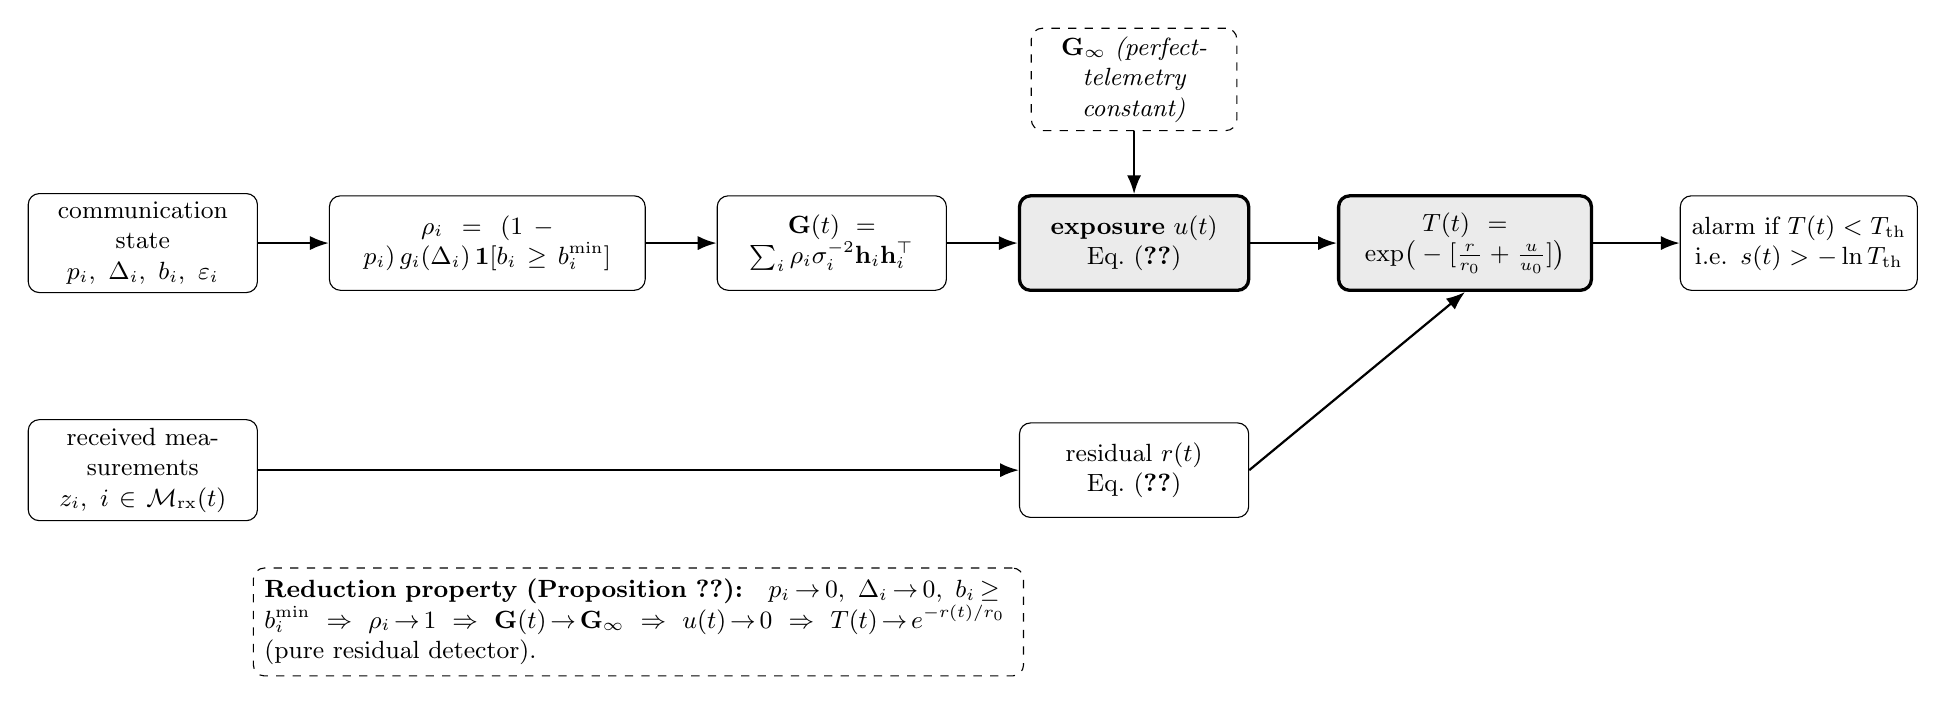
\begin{tikzpicture}[
  >={Latex[length=2.4mm]},
  b/.style={draw,rounded corners,align=center,font=\small,
            inner sep=3pt,fill=white,minimum height=12mm,text width=27mm},
  bb/.style={b,very thick,fill=black!8}]

% ---- top path: communication -> exposure ----
\node[b]                      (comm) at (0,0)
   {communication state\\$p_i,\ \Delta_i,\ b_i,\ \varepsilon_i$};
\node[b, right=9mm of comm,text width=38mm]   (rho)
   {$\rho_i=(1-p_i)\,g_i(\Delta_i)\,\mathbf{1}[b_i\ge b_i^{\min}]$};
\node[b, right=9mm of rho]    (G)
   {$\bG(t)=\sum_i\rho_i\sigma_i^{-2}\bh_i\bh_i^{\top}$};
\node[bb,right=9mm of G]      (u)
   {\textbf{exposure} $u(t)$\\Eq.~\eqref{eq:exposure}};
\node[b, above=8mm of u,dashed,text width=24mm] (Ginf)
   {$\bG_{\infty}$ \emph{(perfect-telemetry constant)}};

% ---- bottom path: measurements -> residual ----
\node[b, below=16mm of comm]  (meas)
   {received measurements\\$z_i,\ i\in\Mrx(t)$};
\node[b]                      (r) at (u|-meas)
   {residual $r(t)$\\Eq.~\eqref{eq:residual}};

% ---- combination ----
\node[bb,right=11mm of u,text width=30mm]    (T)
   {$T(t)=\exp\!\big(-[\tfrac{r}{r_0}+\tfrac{u}{u_0}]\big)$};
\node[b, right=11mm of T,text width=28mm]    (alarm)
   {alarm if $T(t)<T_{\mathrm{th}}$\\
    i.e. $s(t)>-\ln T_{\mathrm{th}}$};

\draw[->,thick] (comm) -- (rho);
\draw[->,thick] (rho)  -- (G);
\draw[->,thick] (G)    -- (u);
\draw[->,thick] (Ginf) -- (u);
\draw[->,thick] (meas) -- (r);
\draw[->,thick] (u)    -- (T);
\draw[->,thick] (r.east) -- (T.south);
\draw[->,thick] (T)    -- (alarm);

\node[draw,dashed,rounded corners,align=left,font=\small,
      inner sep=4pt,text width=95mm] (note) at ($(meas.south)!0.5!(r.south)+(0,-13mm)$)
  {\textbf{Reduction property (Proposition~\ref{prop:reduction}):}\quad
   $p_i\!\to\!0,\ \Delta_i\!\to\!0,\ b_i\!\ge\! b_i^{\min}
   \;\Rightarrow\; \rho_i\!\to\!1
   \;\Rightarrow\; \bG(t)\!\to\!\bG_{\infty}
   \;\Rightarrow\; u(t)\!\to\!0
   \;\Rightarrow\; T(t)\!\to\!e^{-r(t)/r_0}$
   \ \ (pure residual detector).};
\end{tikzpicture}}
\caption{Construction of the communication-aware trust metric and its
reduction to a residual detector under perfect telemetry
(Proposition~\ref{prop:reduction}). Communication resources enter the
trust value through $\rho_i$ and the information matrix, not through the
residual.}
\label{fig:blockdiagram}
\end{figure*}

\subsection{Standing assumptions and regularity conditions}
\label{sec:assumptions}
The following are used by the propositions below and are collected here so
that each can be checked independently.

\begin{assumption}[Perfect-telemetry observability]
\label{as:obs}
$\bG_{\infty}\succ0$, i.e., the full measurement set renders the state
observable~\cite{monticelli1985}. This is what makes $\bG_{\infty}^{-1}$
well defined and the perfect-telemetry floor finite.
\end{assumption}

\begin{assumption}[Bounded state increment]
\label{as:omega}
Between consecutive twin updates the state increment satisfies
$\lVert\bx(t_{k+1})-\bx(t_k)\rVert\le\omega$. We emphasize that $\omega$
is a \emph{per-update increment} in per unit, not a rate in per unit per
second; if a rate $\dot\omega$ is preferred, set
$\omega=\dot\omega\,\bar\Delta$ with $\bar\Delta$ the nominal update
interval. The implemented bound is $\omega=0.02$~p.u. per update.
\end{assumption}

\begin{assumption}[Regularization]
\label{as:eps}
$\epsilon>0$ is fixed and small relative to the informative spectrum of
$\bG_{\infty}$; Table~\ref{tab:hyper} gives the proposed setting. Under
Assumption~\ref{as:obs} the bias introduced by $\epsilon$ vanishes as
$\epsilon\to0$ whenever $\bG(t)\succ0$.
\end{assumption}

\begin{assumption}[Known noise model]
\label{as:noise}
Measurement noise is additive, zero-mean Gaussian, with variances
$\sigma_i^{2}$ frozen in the feeder artifact.
\end{assumption}

\subsection{Properties}
We state structural properties; proofs are short and are given in full.

\begin{proposition}[Range]
\label{prop:range}
$T(t)\in(0,1]$, with $T(t)=1$ if and only if $r(t)=0$ and $u(t)=0$.
\end{proposition}
\begin{IEEEproof}
$r(t)\ge0$ by \eqref{eq:residual} and $u(t)\ge0$ by the $(\cdot)_{+}$
in \eqref{eq:exposure}, so $s(t)\ge0$ and $T=e^{-s}\in(0,1]$. Equality
$T=1$ holds iff $s=0$, i.e., iff both terms vanish. Note $T$ never
attains $0$; the alarm threshold must satisfy
$T_{\mathrm{th}}\in(0,1)$.
\end{IEEEproof}

\begin{proposition}[Residual monotonicity]
\label{prop:resmono}
$T(t)$ is strictly decreasing in $r(t)$.
\end{proposition}
\begin{IEEEproof}
$\partial T/\partial r=-(1/r_0)T<0$ since $T>0$ and $r_0>0$.
\end{IEEEproof}

\begin{proposition}[Communication monotonicity]
\label{prop:commmono}
At fixed $r(t)$, $T(t)$ is nonincreasing as packet loss $p_i$ increases,
as age $\Delta_i$ increases, or as a channel becomes infeasible
($b_i<b_i^{\min}$). Under Assumption~\ref{as:eps} the property holds
unconditionally.
\end{proposition}
\begin{IEEEproof}
Each such change does not increase $\rho_i$ in \eqref{eq:rho}, because
$(1-p_i)$ is nonincreasing in $p_i$, $g$ is nonincreasing, and the
indicator can only switch from $1$ to $0$. Writing $\bG'$ for the
information matrix after the change, $\bG-\bG'=\sum_i(\rho_i-\rho_i')
\sigma_i^{-2}\bh_i\bh_i^{\top}\succeq0$, so $\bG'\preceq\bG$ in the
Loewner order. Hence $\bG'+\epsilon\bI\preceq\bG+\epsilon\bI$, and both
are positive definite, so operator antitonicity of matrix inversion on the
positive-definite cone gives
$(\bG'+\epsilon\bI)^{-1}\succeq(\bG+\epsilon\bI)^{-1}$. Since $\lmax$ is
monotone with respect to the Loewner order,
$\lmax(\bG'_{\epsilon})\ge\lmax(\bG_{\epsilon})$, so $u$ does not decrease
and, by \eqref{eq:trust}, $T$ does not increase. This is the property that
gives the metric its communication awareness. (With the pseudo-inverse in
place of \eqref{eq:regularized} the argument requires the additional
range condition $\operatorname{range}(\bG')=\operatorname{range}(\bG)$, as
noted in Remark~\ref{rem:pinv}, which is precisely what fails under severe
starvation.)
\end{IEEEproof}

\begin{proposition}[Oracle reduction / strict generalization]
\label{prop:reduction}
Under Assumption~\ref{as:obs}, as $p_i\to0$, $\Delta_i\to0$, and
$b_i\ge b_i^{\min}$ for all $i$ (unlimited, timely, loss-free telemetry),
$\rho_i\to1$, $\bG(t)\to\bG_{\infty}$, $u(t)\to0$, and therefore
$T(t)\to\exp(-r(t)/r_0)$---a strictly monotone function of the residual
alone.
\end{proposition}
\begin{IEEEproof}
$p_i\to0$ gives $(1-p_i)\to1$; $\Delta_i\to0$ with $g(0)=1$ and $g$
continuous gives $g(\Delta_i)\to1$; feasibility makes the indicator $1$.
Hence $\rho_i\to1$ and, by \eqref{eq:information},
$\bG(t)\to\bG_{\infty}$ entrywise and therefore in spectrum. Consequently
$\lmax(\bG_{\epsilon}(t))\to\lmax((\bG_{\infty}+\epsilon\bI)^{-1})$, the
bracketed term in \eqref{eq:exposure} tends to $0$ from above, the
$(\cdot)_{+}$ keeps it at $0$, and $u(t)\to0$. Substituting into
\eqref{eq:trust} gives the claim.
\end{IEEEproof}

\begin{corollary}[Exact reduction to the $\chi^{2}$ bad-data test]
\label{cor:exact}
With the normalization of \eqref{eq:residual}, in the perfect-telemetry
limit (in which $g_i\equiv1$) $T(t)=\exp(-J(\bxh)/(m\,r_0))$ where
$J(\bxh)=\sum_{i\in\mathcal{M}}(z_i-\bh_i^{\top}\bxh)^{2}/\sigma_i^{2}$ is
the weighted residual sum of squares of the classical $\chi^{2}$ bad-data
test. The proposed detector and the $\chi^{2}$ test are then \emph{the
same detector} up to a strictly monotone transformation, and therefore
have identical ROC curves.
\end{corollary}

\begin{remark}[The reduction is to $\chi^{2}$, \emph{not} to LNR]
\label{rem:notlnr}
We state this explicitly because it is easy to get wrong. LNR is an
extremum statistic and \eqref{eq:residual} is an aggregate; they are not
monotone transformations of one another and their ROC curves differ.
Corollary~\ref{cor:exact} therefore licenses attributing any measured
ROC difference \emph{against the $\chi^{2}$ baseline} to $u(t)$ alone. The
comparison against LNR is a comparison between two genuinely different
detectors, and a difference there confounds the exposure term with the
aggregate-versus-extremum distinction. Both baselines are reported
(Table~\ref{tab:baselines}); only the $\chi^{2}$ comparison carries the
clean attribution.
\end{remark}

\emph{Consequence, and a distinction that must not be blurred.} Two
different objects appear in this paper and are easily conflated.

\emph{(a) The ideal-telemetry reference} is the $u\equiv0$ regime of the
proposed metric. By Proposition~\ref{prop:reduction} and
Corollary~\ref{cor:exact} it coincides exactly with the $\chi^{2}$ baseline. It
is a \emph{detector}, and it does not know the true state.

\emph{(b) The no-communication-limit oracle} of Section~\ref{sec:setup} is
\emph{not} this object. It additionally observes the true state $\bx(t)$
and hence the true divergence $d(t)$, which no detector can. It is the
ground-truth \emph{labeller} and a performance ceiling, not a competitor
under test.

Conflating (a) and (b) would invalidate the inferential logic of
Section~\ref{sec:results}. Stated correctly: because the metric reduces
exactly to the \emph{$\chi^{2}$} baseline when $u\equiv0$
(Corollary~\ref{cor:exact}, \emph{not} LNR---see
Remark~\ref{rem:notlnr}), any measured ROC difference between the
proposed metric and the $\chi^{2}$ baseline is attributable to $u(t)$
alone \textbf{provided both are computed from the same state estimate}.
That proviso is not cosmetic: since \eqref{eq:estimator} changed the
estimator, a $\chi^{2}$ baseline run on a plain-$\sigma_i^{-2}$ estimate
would differ from the proposed detector for two reasons at once, and the
attribution would fail (Remark~\ref{rem:estmatched}). The oracle plays no
part in that attribution; it supplies labels and an upper reference.

\begin{remark}[All detectors must share one estimator]
\label{rem:estmatched}
Equation~\eqref{eq:estimator} improves the estimate itself, so a detector
fed by it enjoys an advantage that has nothing to do with $u(t)$. In a
controlled check with half the channels fresh and half stale, the
$\chi^{2}$ statistic computed on an age-aware estimate scored an AUC
approximately $0.017$ above the same statistic computed on a plain-WLS
estimate, \emph{with the exposure term absent entirely}. A difference of
that size is well within the resolving power of DeLong's test at the event
counts of Section~\ref{sec:setup}, and would be silently misread as
evidence for the exposure term. We therefore require that \emph{every}
detector under comparison---$\chi^{2}$, LNR, Huber, B1--B3, and the
proposed metric---consume the \emph{same} state estimate from
\eqref{eq:estimator}. We additionally report plain-WLS and native robust
weighting as sensitivity arms so estimator effects remain visible rather
than being absorbed into the proposed statistic.
\end{remark}

\begin{proposition}[Exposure ceiling and alarm feasibility]
\label{prop:ceiling}
Let $L=\lmax((\bG_{\infty}+\epsilon\bI)^{-1})=1/(\lmin(\bG_{\infty})+\epsilon)$,
so that $\nu=1/L$ and \eqref{eq:exposure} may be written
$u(t)=\omega^{2}\big(\lmax(\bG_{\epsilon}(t))/L-1\big)_{+}$. Then the
exposure term is bounded above, with the supremum attained in the
total-starvation limit $\rho_i\to0\ \forall i$:
\begin{equation}
u_{\max}\;=\;\frac{\omega^{2}\,\lmin(\bG_{\infty})}{\epsilon}.
\label{eq:ceiling}
\end{equation}
Consequently, since $r(t)\to0$ under total starvation, a distrust alarm is
raised in that limit \emph{only if}
\begin{equation}
\epsilon\;<\;\frac{\omega^{2}\,\lmin(\bG_{\infty})}{u_0\,\ln(1/T_{\mathrm{th}})}.
\label{eq:epscondition}
\end{equation}
\end{proposition}
\begin{IEEEproof}
As $\rho_i\to0$ for all $i$, $\bG(t)\to\mathbf{0}$, hence
$\bG_{\epsilon}(t)\to\epsilon^{-1}\bI$ and
$\lmax(\bG_{\epsilon}(t))\to\epsilon^{-1}$, its maximum over the
positive-semidefinite cone. Substituting,
\[
u_{\max}=\omega^{2}\!\left(\frac{1}{\epsilon L}-1\right)
=\omega^{2}\!\left(\frac{\lmin(\bG_{\infty})+\epsilon}{\epsilon}-1\right)
=\frac{\omega^{2}\lmin(\bG_{\infty})}{\epsilon}.
\]
An alarm requires $s(t)>-\ln T_{\mathrm{th}}$; with $r=0$ this is
$u_{\max}/u_0>\ln(1/T_{\mathrm{th}})$, which rearranges
to~\eqref{eq:epscondition}.
\end{IEEEproof}

\begin{remark}[Saturation, and why \eqref{eq:epscondition} binds hardest on
the hardest feeders]
\label{rem:saturation}
Proposition~\ref{prop:ceiling} exposes a cost of the regularization
adopted in Remark~\ref{rem:pinv}. True divergence under a prolonged
blackout grows without bound---roughly $k\omega$ after $k$ missed
updates---whereas $u(t)$ saturates at \eqref{eq:ceiling}. Because
$r(t)\to0$ as well, $T(t)$ becomes \emph{constant} during a sustained
blackout: the metric records that the twin is untrustworthy but not that
the situation is deteriorating. For the binary detection task studied here
this is benign, since the alarm is latched once $T$ crosses
$T_{\mathrm{th}}$; for the trust-triggered control that motivates later
work in this thesis, a graded non-saturating signal would be required, and
we flag this explicitly as an open problem
(Section~\ref{sec:discussion}-B). Note also that \eqref{eq:epscondition}
involves $\lmin(\bG_{\infty})$, the information in the \emph{weakest}
observed direction under perfect telemetry. On a weakly observable
unbalanced feeder---precisely the IEEE 123-node case---$\lmin(\bG_{\infty})$
is small, so $\epsilon$ must be small. A default specified relative to
$\lmax(\bG_{\infty})$ can therefore violate \eqref{eq:epscondition} by a
factor of order the condition number $\kappa(\bG_{\infty})$; the setting in
Table~\ref{tab:hyper} is stated relative to $\lmin$ for this reason, and
\eqref{eq:epscondition} is checked numerically before each run.
\end{remark}

\begin{proposition}[$\delta$-confident exposure]
\label{prop:confident}
Condition on the ages and bandwidths, and let the arrival indicators
$a_i\sim\mathrm{Bernoulli}(1-p_i)$ be independent, so that
$\bG_{\mathrm{real}}(t)=\sum_i a_i\gamma_i\mathbf{K}_i$ with
$\gamma_i=g_i(\Delta_i)\mathbf{1}[b_i\ge b_i^{\min}]$,
$\mathbf{K}_i=\sigma_i^{-2}\bh_i\bh_i^{\top}$, and
$\mathbb{E}[\bG_{\mathrm{real}}]=\bG(t)$. Define
\begin{equation}
s_{\delta}(t)=\sqrt{2\,\bar V\log(4n/\delta)}+\tfrac{2}{3}\bar L\log(4n/\delta),
\label{eq:sdelta}
\end{equation}
\begin{equation}
\bar V=\Big\|\sum_i \phi(p_i)\,\mathbf{K}_i^{2}\Big\|,\quad
\bar L=\max_{i:\,p_i>0}\|\mathbf{K}_i\|,\quad
\phi(p)=\begin{cases}p(1-p), & p\le\tfrac12\\[2pt] \tfrac14,& p>\tfrac12,\end{cases}
\label{eq:envelopes}
\end{equation}
where $\phi$ is the nondecreasing envelope of the Bernoulli variance and
$\bar V,\bar L$ deliberately drop the factors $\gamma_i\le1$. These
\emph{envelopes} are what make the bound monotone; the reason is given in
Remark~\ref{rem:monenv}.
and the \emph{loss-quantile} floor
\begin{equation}
\hat\lambda^{\mathrm{Q}}_{\delta}(t)=\Big(\lmin\big(\textstyle\sum_i\gamma_i\mathbf{K}_i\big)
-\Lambda_{k_\delta}\Big)_{+},
\label{eq:quantfloor}
\end{equation}
where $k_\delta$ is the $(1-\delta/2)$ quantile of the Poisson--binomial
number of lost channels and $\Lambda_{k}$ is the sum of the $k$ largest
\emph{unweighted} norms $\|\mathbf{K}_i\|$ (again dropping
$\gamma_i\le1$, for the same reason). Define the \textbf{combined floor}
\begin{equation}
\hat\lambda_{\delta}(t)=\max\Big\{
\big(\lmin(\bG(t))-s_{\delta}(t)\big)_{+},\;
\hat\lambda^{\mathrm{Q}}_{\delta}(t)\Big\},
\label{eq:combfloor}
\end{equation}
each constituent evaluated at level $\delta/2$. Then with probability at
least $1-\delta$ over the arrivals,
\begin{equation}
\lmax\!\big((\bG_{\mathrm{real}}(t)+\epsilon\bI)^{-1}\big)\;\le\;
\frac{1}{\hat\lambda_{\delta}(t)+\epsilon}.
\label{eq:confbound}
\end{equation}
Replacing $\lmax(\bG_{\epsilon}(t))$ in \eqref{eq:exposure} by the
right-hand side of \eqref{eq:confbound} yields an exposure
$u^{\delta}(t)$ that is, with confidence $1-\delta$, an \emph{upper} bound
on the realized worst-direction posterior variance rather than an
optimistic mean-based proxy. Moreover $\hat\lambda_{\delta}$ is
nonincreasing under any communication degradation---increase of any $p_i$,
increase of any $\Delta_i$, or loss of bandwidth feasibility---so
$u^{\delta}$ inherits Proposition~\ref{prop:commmono}. Finally
$\hat\lambda_{\delta}(t)\to\lmin(\bG_{\infty})$ as $p_i\to0$, $\Delta_i\to0$,
$b_i\ge b_i^{\min}$; hence $u^{\delta}\to0$ and
Propositions~\ref{prop:commmono} and~\ref{prop:reduction} and
Corollary~\ref{cor:exact} carry over \emph{in the limit}, not merely at
the isolated point $p\equiv0$.
\end{proposition}
\begin{IEEEproof}
Let $\mathbf{S}_i=(a_i-(1-p_i))\gamma_i\mathbf{K}_i$; these are
independent, self-adjoint, and centered, with
$\|\mathbf{S}_i\|\le L$ almost surely and
$\|\sum_i\mathbb{E}\mathbf{S}_i^{2}\|=V$ (channels with
$p_i\in\{0,1\}$ satisfy $\mathbf{S}_i\equiv0$ and are excluded from the
maximum defining $L$). The matrix Bernstein inequality gives
$\|\bG_{\mathrm{real}}-\bG\|\le s_{\delta}$ with probability at least
$1-\delta$. On that event, Weyl's inequality yields
$\lmin(\bG_{\mathrm{real}})\ge\lmin(\bG)-s_{\delta}$, and since
$\lmin(\bG_{\mathrm{real}})\ge0$ always, also
$\|\mathbf{S}_i\|\le\gamma_i\|\mathbf{K}_i\|\le\bar L$ and
$\|\sum_i\mathbb{E}\mathbf{S}_i^{2}\|
=\|\sum_i p_i(1-p_i)\gamma_i^{2}\mathbf{K}_i^{2}\|\le\bar V$, since
$\gamma_i\le1$ and $p(1-p)\le\phi(p)$; the envelopes therefore only
enlarge the deviation bound and \eqref{eq:sdelta} remains valid. Matrix
Bernstein and Weyl then give
$\lmin(\bG_{\mathrm{real}})\ge(\lmin(\bG)-s_{\delta})_{+}$ at level
$\delta/2$. For the second constituent, at most $k_{\delta}$ channels are
lost with probability $1-\delta/2$, and on that event
$\bG_{\mathrm{real}}\succeq\sum_i\gamma_i\mathbf{K}_i-\sum_{i\in\mathcal{S}}\gamma_i\mathbf{K}_i$
for some $|\mathcal{S}|\le k_{\delta}$, whence
$\lmin(\bG_{\mathrm{real}})\ge\lmin(\sum_i\gamma_i\mathbf{K}_i)-\Lambda_{k_\delta}$
by Weyl. A union bound gives both simultaneously with probability
$1-\delta$, so $\lmin(\bG_{\mathrm{real}})\ge\hat\lambda_{\delta}$ and
\eqref{eq:confbound} follows. For the limit claim: as $p_i\to0$ we have
$k_{\delta}\to0$, hence $\Lambda_{k_\delta}\to0$ and
$\hat\lambda^{\mathrm{Q}}_{\delta}\to\lmin(\sum_i\gamma_i\mathbf{K}_i)$,
which tends to $\lmin(\bG_{\infty})$ as $\gamma_i\to1$. For monotonicity, treat the two constituents separately.
$\hat\lambda^{\mathrm{Q}}_{\delta}$: the matrix $\sum_i\gamma_i\mathbf{K}_i$
is Loewner-nonincreasing as any $\gamma_i$ falls, so its $\lmin$ is
nonincreasing; $\Lambda_{k}$ is now $\gamma$-free and nondecreasing in
$k$, and $k_{\delta}$ is nondecreasing in every $p_i$; hence the
difference is nonincreasing. $(\lmin(\bG)-s_{\delta})_{+}$: the matrix
$\bG=\sum_i(1-p_i)\gamma_i\mathbf{K}_i$ is Loewner-nonincreasing in every
$p_i$ and $\gamma_i$; $\bar V$ is $\gamma$-free and nondecreasing in each
$p_i$ because $\phi$ is nondecreasing; and $\bar L$ is $\gamma$-free and
nondecreasing because the index set $\{i:p_i>0\}$ only grows. Hence
$s_{\delta}$ is nondecreasing and the difference nonincreasing. The
maximum of two nonincreasing functions is nonincreasing.
\end{IEEEproof}

\begin{remark}[Why the envelopes are necessary, and what they cost]
\label{rem:monenv}
It is tempting to use the tightest available deviation bound---to retain
the factors $\gamma_i$ in $V$ and $L$ and the exact Bernoulli variance
$p_i(1-p_i)$. Doing so \emph{destroys monotonicity}, in a direction that
matters. Consider degrading a single channel $i$ whose
$\|\mathbf{K}_i\|$ is large but whose measurement direction is
well-observed, so $\lmin(\bG)$ barely moves. A $\gamma$-weighted deflation
shrinks with $\gamma_i$, so the floor $\lmin(\bG)-s_{\delta}$
\emph{rises}, $u^{\delta}$ \emph{falls}, and the metric reports
\emph{increasing} trust as the link degrades---exactly the pathology
Proposition~\ref{prop:commmono} exists to exclude. The same mechanism
operates through $p_i(1-p_i)$, which decreases once $p_i$ passes
$\tfrac12$. The envelopes of \eqref{eq:envelopes}, together with the
$\gamma$-free $\Lambda_k$, remove both effects by making every deflation
term nondecreasing under degradation.

The cost is conservatism, governed by the heterogeneity of the channel
norms, since $\bar L=\max_i\|\mathbf{K}_i\|$ replaces a $\gamma$-weighted
maximum. Where channel norms are comparable the penalty is slight; where a
single channel dominates the norm spectrum, $\bar L$ is set by that
channel and the floor can collapse. We therefore report the
norm-heterogeneity diagnostic
$\max_i\|\mathbf{K}_i\|/\mathrm{median}_i\|\mathbf{K}_i\|$ for the IEEE
123-node measurement set alongside the deflation ratio.
\end{remark}

\begin{remark}[Why the second constituent is necessary]
\label{rem:whyquantile}
The Bernstein constituent alone is \emph{discontinuous} at $p\equiv0$: its
almost-sure term $L$ does not vanish as $p_i\to0^{+}$ (a loss of
probability $p_i$ still has magnitude $\approx\gamma_i\|\mathbf{K}_i\|$
when it occurs), so $s_{\delta}$ jumps from $0$ to a value that can exceed
$\lmin(\bG)$ the instant any $p_i>0$. Used alone it would therefore
satisfy the reduction property only \emph{at} $p\equiv0$ and not in the
limit---which is the sense in which
Proposition~\ref{prop:reduction} is stated, and hence not good enough. The
loss-quantile constituent \eqref{eq:quantfloor} is exact at $p\equiv0$
($k_\delta=0$) and remains exact on a neighbourhood
($\sum_ip_i\lesssim\delta$), repairing the limit. Conversely
\eqref{eq:quantfloor} degrades quickly once $k_\delta$ grows, where
Bernstein is far tighter. The maximum \eqref{eq:combfloor} inherits the
better of the two everywhere and is what we use.
\end{remark}

\begin{remark}[When \eqref{eq:confbound} is informative, and a tighter
practical variant]
\label{rem:tightness}
Both constituents of \eqref{eq:combfloor} are uniform over directions and
therefore conservative: $s_{\delta}$ scales as $\sqrt{V\log n}$ while
$\lmin(\bG)$ scales with the redundancy $m/n$, so on measurement sets of
low redundancy the combined floor can still collapse to zero, in which
case $u^{\delta}$ saturates at the ceiling of
Proposition~\ref{prop:ceiling}. We therefore report the \emph{deflation
ratio} $s_{\delta}/\lmin(\bG)$, the quantile $k_\delta$, the
norm-heterogeneity diagnostic of Remark~\ref{rem:monenv}, and which
constituent is active, for the IEEE 123-node measurement set. If both
constituents floor at zero across all regimes, $u^{\delta}$ carries no
gradient; we then report the mean form $u$ as primary and $u^{\delta}$ as
a conservative check, and say so explicitly.

A materially tighter practical variant fixes the direction: let
$\hat{\mathbf{v}}$ be the unit eigenvector of $\bG(t)$ for
$\lmin(\bG(t))$ and apply the \emph{scalar} Bernstein inequality to
$\hat{\mathbf{v}}^{\top}\bG_{\mathrm{real}}\hat{\mathbf{v}}
=\sum_i a_i\gamma_i\kappa_i$, $\kappa_i=\hat{\mathbf{v}}^{\top}\mathbf{K}_i\hat{\mathbf{v}}\ge0$,
which removes the dimension factor $n$ and replaces $V$ by
$\sum_i p_i(1-p_i)\gamma_i^2\kappa_i^{2}$. We emphasize that this variant
is \emph{not} a uniform guarantee, because the minimizing direction is
itself random and $\lmin(\bG_{\mathrm{real}})\le
\hat{\mathbf{v}}^{\top}\bG_{\mathrm{real}}\hat{\mathbf{v}}$; its
attained coverage is therefore an empirical quantity, and we report
measured coverage alongside the nominal $1-\delta$
(Table~\ref{tab:sensitivity}). Both variants are swept.
\end{remark}

\begin{proposition}[Silent-drift sensitivity --- central empirical hypothesis]
\label{prop:hypothesis}
Suppose true divergence grows ($d(t)>\gamma$) during an interval in which
channels are starved so that $\rho_i$ is small and the received residual
stays below the classical threshold ($r(t)<\eta$). Then $u(t)>0$ and
$T(t)$ is strictly reduced relative to its unstarved value, yielding a
distrust alarm where a residual-only detector remains silent.
\end{proposition}

\noindent\textbf{Status of Proposition~\ref{prop:hypothesis}.} This is the
property the paper \emph{tests}, not a theorem we assert. The forward
implication ``starvation $\Rightarrow u>0 \Rightarrow T$ reduced'' follows
from Proposition~\ref{prop:commmono}; what is \emph{not} guaranteed is
that the reduction is large enough, and timely enough, to separate
silent-drift events from nominal operation at a useful false-alarm rate,
since that depends on Assumption~\ref{as:omega}, on the observability
geometry, and on the calibration of $r_0,u_0,T_{\mathrm{th}}$. We
therefore treat Proposition~\ref{prop:hypothesis} as a hypothesis to be
validated in Sections~\ref{sec:setup}--\ref{sec:results}.

\subsection{Relationship to residuals and age}
The residual term $r(t)$ coincides (up to the normalization noted in
Remark~\ref{rem:residual}) with the statistic used by bad-data
detection~\cite{abur2004,handschin1975,gol2014lav}; the age variables
$\Delta_i$ subsume the information used by age-based
qualifiers~\cite{duran2023,cosandal2026}. The novelty is neither term in
isolation but (i) the exposure term $u(t)$ that maps communication
scarcity through the measurement model into an undetected-divergence bound
and (ii) the reduction property (Proposition~\ref{prop:reduction}) that
makes the metric a strict generalization of residual detection.

% =====================================================================
\section{Experimental Setup}
\label{sec:setup}

\subsection{Test feeder}
We use the IEEE 123-node distribution test
feeder~\cite{kersting1991,ieee123,dugan2009}. The OpenDSS exporter
preserves its unbalanced multiphase topology, regulators, capacitors,
switches, and phase-specific loads, then maps the solved circuit to a
frozen linearized model with $n=491$ states and $m=583$ measurements. Of
these, 45 are communicated telemetry channels and 538 are local
pseudo-measurements. The exported matrix, channel ordering, covariance
model, process matrix $\bQ$, and divergence weight $\bW=\bI_{491}$ are
immutable inputs to calibration and evaluation. This fixed, highly
anisotropic measurement geometry is the object tested by the exposure
term; it is not re-estimated from evaluation outcomes.

\subsection{Co-simulation stack}
The physical trajectories are solved offline by OpenDSS and sealed as
seeded, label-free truth artifacts. A HELICS co-simulation
\cite{palmintier2017,hardy2024} then connects four production federates:
(i) a power federate that streams noisy telemetry packets from the frozen
truth; (ii) an ns-3.35 network federate that applies bandwidth, delay,
random loss, starvation, and queueing; (iii) a Python twin federate that
runs the age-aware estimator and computes all detector statistics; and
(iv) an oracle federate that receives the twin output and assigns
evaluation labels from the inaccessible true state. A HELICS broker
coordinates logical time. Network impairments therefore alter only
telemetry delivery, while paired methods within a cell share the same
physical trajectory and measurement-noise realization. Fig.~\ref{fig:cosim}
shows the arrangement.

\subsection{Computational cost}
The production implementation forms a row-scaled information matrix and
uses a dense singular-value decomposition to obtain the spectrum once per
update; that one spectrum serves the mean and conservative exposure forms
and both $\lmax$ and trace scalarizations. Perfect-telemetry spectra and
normalizers are precomputed. We do not infer real-time feasibility from
asymptotic complexity alone: the confirmatory output reports wall-clock
time per update and peak memory from the pinned container.

\subsection{Reproducibility and version pin}
The network simulator is pinned to \textbf{ns-3.35}. This is required
because the \texttt{helics-ns3} integration module uses the WAF
contributed-build system, whereas ns-3 switched from WAF to CMake at
version 3.36, which breaks the module; the project documentation states
that the module will not work with ns-3.36 or newer~\cite{helicsns3}. We
report HELICS \textbf{v3.6.1}. The artifact package records container,
source, input, and output SHA-256 digests; run metadata are accepted only
when all four federates report status \texttt{complete} and the declared
cardinalities.

\subsection{Physical trajectories and event design}
For each physical seed, the OpenDSS exporter produces 1,100 independent
12-step trajectories (13,200 one-second steps). The predeclared physical
event allocation is 605 nominal, 198 load-ramp, 165 parameter-change, and
132 topology-change events. Load ramps alter selected downstream load
groups by a seeded magnitude and direction; parameter changes apply
seeded regulator-tap perturbations; and topology changes operate one of
the predeclared study ties. Background load, photovoltaic, cloud,
motor-load, and diurnal variations are seeded independently. The
evaluation artifacts contain no detector-derived label, and evaluation
trajectory identifiers are disjoint from calibration.

\begin{figure}[!t]
\centering
\resizebox{0.99\columnwidth}{!}{%
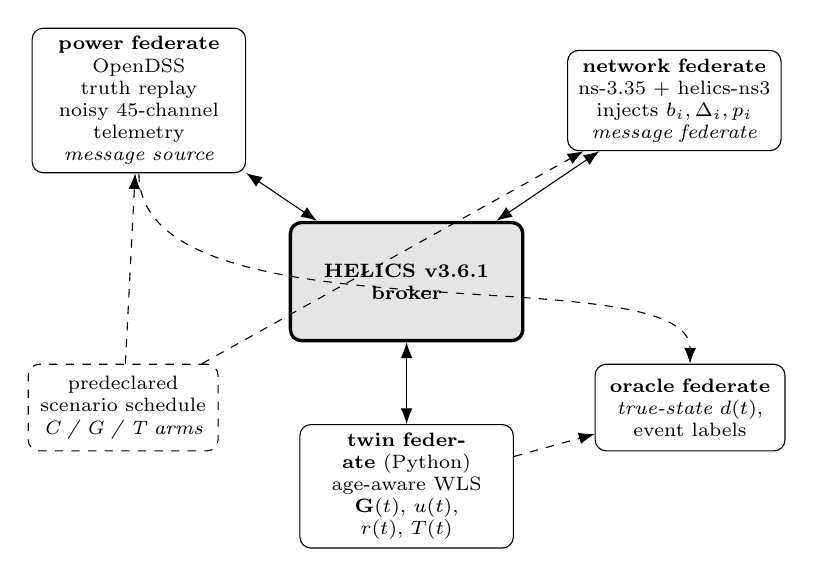
\begin{tikzpicture}[
  >={Latex[length=2mm]},
  f/.style={draw,rounded corners,align=center,font=\scriptsize,
            inner sep=3pt,fill=white,minimum height=11mm,text width=25mm},
  hub/.style={draw,very thick,rounded corners,align=center,
              font=\scriptsize\bfseries,fill=black!10,inner sep=5pt,
              text width=26mm,minimum height=15mm}]

\node[hub] (broker) at (0,0) {HELICS v3.6.1\\broker};

\node[f] (power) at (-3.4,2.3)
  {\textbf{power federate}\\OpenDSS truth replay\\noisy 45-channel
   telemetry\\{\itshape message source}};
\node[f] (net) at (3.4,2.3)
  {\textbf{network federate}\\ns-3.35 + helics-ns3\\injects
   $b_i,\Delta_i,p_i$\\{\itshape message federate}};
\node[f] (twin) at (0,-2.6)
  {\textbf{twin federate} (Python)\\age-aware WLS\\
   $\bG(t)$, $u(t)$, $r(t)$, $T(t)$};

\node[f,dashed,text width=22mm] (drift) at (-3.6,-1.6)
  {predeclared\\scenario schedule\\{\itshape C / G / T arms}};
\node[f,text width=22mm] (oracle) at (3.6,-1.6)
  {\textbf{oracle federate}\\{\itshape true-state} $d(t)$,\\event labels};

\draw[<->] (broker) -- (power);
\draw[<->] (broker) -- (net);
\draw[<->] (broker) -- (twin);
\draw[->,dashed] (drift) -- (power);
\draw[->,dashed] (drift) -- (net);
\draw[->,dashed] (power.south) .. controls +(0,-2.2) and +(0,1.4) .. (oracle.north);
\draw[->,dashed] (twin) -- (oracle);
\end{tikzpicture}}
\caption{Four-federate HELICS co-simulation. The power federate streams
OpenDSS-derived truth through ns-3.35 to the estimator/metric federate;
the oracle labels its output from the inaccessible true state. Telemetry
degradation is applied only on the message path, so paired comparisons
within a seed use the same physical trajectory.}
\label{fig:cosim}
\end{figure}

\begin{table}[!t]
\caption{Predeclared bandwidth factor (experimental configuration).}
\label{tab:regimes}
\centering
\footnotesize
\renewcommand{\arraystretch}{1.2}
\begin{tabular}{@{}l r p{3.6cm}@{}}
\toprule
Level & Aggregate cap & Purpose \\
\midrule
\texttt{bw00\_floor} & $0.5$ bit/s & total-starvation stress limit \\
\texttt{bw01\_10kbps} & $10^{4}$ bit/s & constrained telemetry \\
\texttt{bw02\_100kbps} & $10^{5}$ bit/s & intermediate telemetry \\
\texttt{bw03\_1mbps} & $10^{6}$ bit/s & high-bandwidth telemetry \\
\texttt{bw04\_oracle} & $10^{12}$ bit/s & practically unconstrained network control \\
\bottomrule
\end{tabular}
\\[2pt]
\begin{minipage}{0.98\columnwidth}
\footnotesize
Each of the 30 unseen physical seeds is evaluated at all five levels,
giving 150 paired cells. The within-run G arm additionally contains 200
events each in ample, moderate, and severe starvation regimes; Arm C has
300 cardinality/age-matched events and Arm T has 200 total-starvation
events. Age, random loss, and starved-channel identity are recorded
outcomes of the ns-3/scenario process rather than substituted nominal
ranges.
\end{minipage}
\end{table}

\begin{table}[!t]
\caption{Baseline methods and their blind spots.}
\label{tab:baselines}
\centering
\footnotesize
\renewcommand{\arraystretch}{1.2}
\begin{tabular}{@{}l p{2.3cm} p{2.4cm}@{}}
\toprule
Method & Detection statistic & Expected blind spot \\
\midrule
\multicolumn{3}{@{}l}{\emph{Reference (not a competitor)}}\\
Oracle labeller & true divergence $d(t)$ & none; requires $\bx(t)$, not deployable \\
\midrule
\multicolumn{3}{@{}l}{\emph{Classical (evidence-driven)}}\\
$\chi^{2}$ bad-data~\cite{abur2004,handschin1975} & $J(\bxh)$, weighted
residual sum of squares & quiet when evidence is absent; \textbf{exact
$u\!\equiv\!0$ limit of the proposed metric} (Cor.~\ref{cor:exact}) \\
LNR bad-data~\cite{abur2004,handschin1975} & largest normalized residual
& quiet when evidence is absent; extremum, \emph{not} a monotone map of
$r(t)$ (Remark~\ref{rem:notlnr}) \\
Huber robust SE~\cite{gol2014lav,abur2004} & robust weighted residual & quiet when evidence is absent \\
\midrule
\multicolumn{3}{@{}l}{\emph{Trivial communication-aware (\textbf{new; the decisive controls})}}\\
B1 Received fraction & $|\Mrx(t)|/m$ & ignores \emph{which} channels and observability geometry \\
B2 Mean age & $\bar\Delta(t)$ & ignores loss and geometry \\
B3 AoT / AoI proxy~\cite{duran2023,yates2021} & worst-case age & age $\ne$ divergence bound \\
\midrule
\textbf{Proposed} & $s(t)=r/r_0+u/u_0$ & weak-observability direction with no drift (Remark~\ref{rem:direction}) \\
\bottomrule
\end{tabular}
\end{table}

\subsection{Drift-injection protocol}
Each cell replays the 1,100 physical events through one bandwidth level.
The physical family and communication pattern are generated independently:
the experiment does not tune starvation to keep the residual below
$\eta$. Residual silence is measured afterward according to
Definition~\ref{def:silentdrift}, which preserves F1 as a falsifiable
quantity. The event table contains three predeclared arms: G (600 events;
200 each in ample, moderate, and severe communication regimes), C (300
events; cardinality- and age-matched measurement-identity contrasts), and
T (200 total-starvation stress events). Every event has 12 one-second
steps. Channel identities and loss/age realizations are fixed by the
scenario table and seed before detector scores are evaluated, preventing
selection on the proposed metric's outcome.

\subsection{Baselines, including the decisive trivial controls}
Table~\ref{tab:baselines} lists the comparison set. The \textbf{oracle
labeller} observes the true state and hence $d(t)$; it supplies the drift
labels of Definition~\ref{def:driftevent} and an upper performance
reference, and---per the distinction drawn after
Corollary~\ref{cor:exact}---is not itself a competitor. The
\textbf{classical} baselines are the $\chi^{2}$ test (primary,
per Corollary~\ref{cor:exact}), LNR bad-data
detection~\cite{abur2004,handschin1975}, and Huber robust
state-estimation residuals~\cite{gol2014lav,abur2004}. \emph{All detectors
consume the same age-aware state estimate} \eqref{eq:estimator}; a
plain-WLS arm is reported separately so the estimator effect is visible
rather than absorbed into the exposure term
(Remark~\ref{rem:estmatched}).

Beyond these we add three \textbf{trivial communication-aware} statistics
(B1--B3), which we regard as the most important comparison in the paper.
The obvious null hypothesis is that the exposure construction is
unnecessary---that simply counting how many channels reported (B1), or how
stale they are (B2--B3), captures whatever advantage communication
awareness confers. Proposition~\ref{prop:cardinality} makes precise when
that null hypothesis must fail, and thereby turns F3 from a coin flip into
a designed test.

\begin{proposition}[Cardinality-blindness of the trivial statistics]
\label{prop:cardinality}
B1 depends on the communication state only through $|\Mrx(t)|$, and B2
only through $\bar\Delta(t)$. Hence for any two configurations $c,c'$ with
$|\Mrx(c)|=|\Mrx(c')|$ and $\bar\Delta(c)=\bar\Delta(c')$, B1 and B2
assign \emph{identical} scores, whereas
$u(c)\neq u(c')$ whenever $\lmin(\bG(c))\neq\lmin(\bG(c'))$. Consequently,
if a fraction $q$ of positive--negative event pairs in the evaluation set
is matched in this way, then
\begin{equation}
\mathrm{AUC}_{\mathrm{B1}}\;\le\;1-\tfrac{q}{2},
\label{eq:aucceiling}
\end{equation}
while the proposed metric is subject to no such ceiling.
\end{proposition}
\begin{IEEEproof}
The first claim is immediate since B1 and B2 are functions of
$|\Mrx|$ and $\bar\Delta$ alone, whereas $u$ depends on $\bG$, which
depends on \emph{which} channels are received through
$\sum_i\rho_i\sigma_i^{-2}\bh_i\bh_i^{\top}$. For \eqref{eq:aucceiling},
recall $\mathrm{AUC}=\Pr(s^{+}>s^{-})+\tfrac12\Pr(s^{+}=s^{-})$. Matched
pairs are ties and contribute $\tfrac12$ each; the remaining $1-q$ of
pairs contribute at most $1$. Hence
$\mathrm{AUC}\le(1-q)+\tfrac{q}{2}=1-\tfrac{q}{2}$.
\end{IEEEproof}

Proposition~\ref{prop:cardinality} identifies the precise locus of the
contribution: the exposure term earns its complexity only insofar as
\emph{which} channels are starved matters, not merely \emph{how many}. A
concrete instance makes the gap vivid. On a feeder where one state
direction is observed by only a few channels, starving that handful
collapses $\lmin(\bG)$ while starving the same number of redundant
channels barely perturbs it; B1 is identical in both cases by
construction, and $u$ can differ by orders of magnitude.

\textbf{Quantitative expectation.} Proposition~\ref{prop:cardinality} is
qualitative; controlled checks make the magnitude concrete and give the
experiment a falsifiable prediction. On a measurement set whose channels
are near-homogeneous, so that $\lmin(\bG)$ is essentially a function of
how many channels report, the exposure term earned \emph{no} premium over
the hybrid $s^{\mathrm{B1}}$---indeed a slightly negative one. On a set
containing a direction observed by only a few channels, the premium was
clearly positive. The value of the information-geometric construction is
therefore \emph{contingent on the observability heterogeneity of the
feeder}, not intrinsic to the construction. We accordingly report, for the
IEEE 123-node measurement set, the spread of per-channel leverage
$\|\mathbf{K}_i\|$ and the sensitivity of $\lmin(\bG)$ to removal of each
single channel, so a reader can judge in advance whether the feeder is of
the kind on which $u$ can help.

\textbf{Protocol consequence, and a guard against rigging.} Since $q$ is a
property of the drift-injection design, we must not simply choose $q$ to
manufacture a favourable F3 verdict---that would repeat, in a subtler
form, the circularity removed in Remark~\ref{rem:circularity}. We
therefore run \emph{two} pre-registered arms and report both:
\begin{itemize}
\item \textbf{Arm C (cardinality-only control), $q=1$.} Starvation
patterns are drawn so that positives and negatives are matched in received
count and mean age. Here \eqref{eq:aucceiling} forces
$\mathrm{AUC}_{\mathrm{B1}}\le0.5$, and any advantage of the proposed
metric is attributable purely to observability geometry.
\item \textbf{Arm G (geometry-varied), $q$ measured.} Starvation patterns
are drawn from a realistic model of correlated link failure, so $q$ is
whatever the physical scenario produces rather than whatever we choose.
\end{itemize}
Arm G is the honest test of F3; Arm C isolates the mechanism. We report
the measured $q$ for Arm G alongside every F3 verdict, so a reader can
compute the ceiling \eqref{eq:aucceiling} independently. If the proposed
metric beats B1 only in Arm C and not in Arm G, the correct conclusion is
that the information-geometric structure is real but operationally
irrelevant for realistic failure patterns---and we will report that.

\subsection{Metrics}
\begin{itemize}
\item \textbf{Silence rate $S$} (Definition~\ref{def:silentdrift}): the
measured fraction of drift events that are residual-silent, per regime.
This quantifies whether the phenomenon motivating the paper actually
occurs, and at what rate.
\item \textbf{Drift-detection latency:} time from onset of a labelled
drift event to the first distrust alarm.
\item \textbf{False-alarm rate (FAR)} and \textbf{missed-drift rate} as
functions of packet loss, compared at \emph{matched FAR}.
\item \textbf{ROC curves swept over communication bandwidth}, summarized
by AUC at each bandwidth level. Per Remark~\ref{rem:roc}, ROC computation
uses $s(t)$ directly.
\end{itemize}

\noindent\textbf{Unit of statistical analysis.} Detection time series are
strongly autocorrelated within an event, so treating individual timesteps
as independent samples would inflate the effective sample size and render
$p$-values meaningless. The unit of analysis is therefore the
\textbf{event}: each drift event and each matched nominal interval
contributes exactly one score, taken as the maximum of its 12 step-level
scores. Confidence intervals use a cluster bootstrap resampling
\emph{seeds} (not timesteps), so that within-seed correlation is
preserved.

\subsection{Separability test and falsification criterion}
For each bandwidth level we compare the ROC/AUC of the proposed metric
against the residual-based detector. The primary inferential quantity is
the within-seed AUC difference: physical seeds are paired, uncertainty is
estimated with a 2,000-resample seed-cluster bootstrap, and a paired
Wilcoxon test is reported. Multiple-comparison correction across bandwidth
levels uses the Holm--Bonferroni procedure~\cite{holm1979}. A pooled-event
DeLong comparison~\cite{delong1988,sun2014} is retained only as a
secondary implementation cross-check because it does not replace
seed-clustered inference. Implementations are cross-checked with
\texttt{pROC}~\cite{robin2011} in R (Table~\ref{tab:tools}).

\begin{quote}
\textbf{Pre-registered falsification criteria.} The contribution must
survive \emph{all three} of the following, each of which can independently
fail.

\textbf{F1 (phenomenon).} If the measured silence rate $S$ is negligible
even under severe starvation---that is, if drift events are almost always
accompanied by a residual alarm---then silent drift is not an
operationally significant phenomenon and the motivation for the metric
collapses, regardless of detector performance.

\textbf{F2 (separability from the classical baseline).} The primary
comparator is the $\chi^{2}$ test, because
Corollary~\ref{cor:exact} makes it the exact $u\equiv0$ limit of the
proposed metric and therefore the only comparison whose difference is
attributable to $u(t)$ alone; LNR and Huber are reported alongside as
secondary, confounded comparisons (Remark~\ref{rem:notlnr}). The comparison must be
\textbf{estimator-matched}: the $\chi^{2}$ detector is computed from the
same age-aware estimate \eqref{eq:estimator} as the proposed metric, so
that the difference isolates $u(t)$ (Remark~\ref{rem:estmatched}). If the
proposed metric's ROC is statistically indistinguishable from the
estimator-matched $\chi^{2}$ detector across the bandwidth sweeps after
Holm--Bonferroni correction, the metric is not separable and the
contribution fails. Validation requires a significant
advantage at low bandwidth / high loss / high age \emph{and} convergence
toward the baseline as communication approaches the ideal-telemetry
regime, as predicted by Proposition~\ref{prop:reduction} and
Corollary~\ref{cor:exact}.

\textbf{F3 (necessity of the information-geometric structure).} The
comparison is against the \textbf{hybrid} statistics
$s^{\mathrm{B1}}=r/r_0+\beta_1(1-|\Mrx|/m)$ and
$s^{\mathrm{B2}}=r/r_0+\beta_2\bar\Delta$, which replace $u$ by a trivial
communication statistic \emph{inside the same combination}, with
$\beta_j$ tuned in the baselines' favour. Comparing the full metric
against \emph{bare} B1 would confound the contribution of $u$ with that of
the residual term, since bare B1 carries no measurement evidence at all;
the hybrid isolates $u$. If $s^{\mathrm{B1}}$ or $s^{\mathrm{B2}}$
achieves AUC statistically indistinguishable from $s$ at matched FAR
\emph{in Arm G}, the exposure construction is unnecessary overhead for
realistic failure patterns; we will report that negative result and
re-scope around the simpler statistic rather than retaining
\eqref{eq:exposure}. Arm C is reported
alongside as a mechanism check, where
Proposition~\ref{prop:cardinality} guarantees
$\mathrm{AUC}_{\mathrm{B1}}\le0.5$; passing Arm C alone does \emph{not}
constitute passing F3.

F3 is stated deliberately: it is the criterion most likely to fail, and
the one whose omission would most weaken the paper.
\end{quote}

\begin{table}[!t]
\caption{Software and tools used to run the experiments and generate the
figures.}
\label{tab:tools}
\centering
\footnotesize
\renewcommand{\arraystretch}{1.2}
\begin{tabular}{@{}p{1.9cm} p{3.0cm} p{2.2cm}@{}}
\toprule
Component & Tool (version) & Role \\
\midrule
Co-simulation & HELICS v3.6.1~\cite{palmintier2017,hardy2024} & federate
orchestration, time sync \\
Physical truth & OpenDSS, pinned exporter image & seeded unbalanced feeder
trajectories \\
Network & ns-3.35 + \texttt{helics-ns3}~\cite{nsnam,helicsns3} &
bandwidth, latency, loss injection \\
State estimation & Python/NumPy/SciPy, with \textbf{age-aware weights}
$g_i\sigma_i^{-2}$ per Eq.~\eqref{eq:estimator} & $\bxh(t)$, residuals \\
Metric computation & NumPy / SciPy & $\bG(t)$, $\bG_{\infty}$,
eigenvalues, $u(t)$, $T(t)$ \\
ROC / AUC / inference & pandas/SciPy seed-level AUC and paired bootstrap;
\texttt{pROC} DeLong cross-check~\cite{robin2011,delong1988,sun2014} & confirmatory figures and tables \\
Correction & Holm--Bonferroni~\cite{holm1979} (statsmodels) &
five-level multiplicity control \\
Plots / tables & matplotlib / pandas & publication PDF/PNG/CSV/TeX outputs \\
Diagrams & Ti\emph{k}Z & Figs.~\ref{fig:concept}--\ref{fig:cosim} \\
\bottomrule
\end{tabular}
\end{table}

\begin{table}[!t]
\caption{Pre-registered sensitivity analysis. Each row is swept with all
other settings held at their Table~\ref{tab:hyper} defaults.}
\label{tab:sensitivity}
\centering
\footnotesize
\renewcommand{\arraystretch}{1.2}
\begin{tabular}{@{}l p{2.5cm} p{2.4cm}@{}}
\toprule
Swept quantity & Range & Question addressed \\
\midrule
$\bQ$ scale & $\pm$ one order of magnitude & sensitivity of the derived
$\tau_i$, which now enters \emph{both} $u$ and $r$
(Lemma~\ref{lem:age}, Remark~\ref{rem:ageconsistent}) \\
Residual weighting & $g_i$-weighted / unweighted & verifies the
age-consistency correction; unweighted should show age-driven FAR \\
Estimator weights & age-aware \eqref{eq:estimator} / plain $\sigma_i^{-2}$
& Remark~\ref{rem:estcoupling}: plain weights break both $u$ and $r$;
report $\|\mathrm{cov}(\bxh-\bx)-\bG^{-1}\|/\|\bG^{-1}\|$ \\
Estimator matching & all detectors on one estimate / native per detector &
Remark~\ref{rem:estmatched}: quantify the estimator-only AUC shift \\
Combination form & additive / coverage-gated $\pi(|\Mrx|/m)$ &
Remark~\ref{rem:antiinformative}: $r$ can be anti-informative under
starvation \\
Feeder heterogeneity & report spread of $\|\mathbf{K}_i\|$ and
single-channel sensitivity of $\lmin(\bG)$ & determines whether $u$ can
outperform B1 at all (Prop.~\ref{prop:cardinality}) \\
$\delta$ & $0.01$--$0.10$ & conservatism of $u^{\delta}$; report deflation
ratio $s_\delta/\lmin(\bG)$ and measured coverage \\
$\omega$ & $\pm$ one order of magnitude & robustness of the increment bound \\
$\epsilon$ & spanning \eqref{eq:epscondition} boundary & does the alarm
survive the feasibility limit? \\
$\gamma$, $\eta$ & $\pm50\%$ & construct validity of the labels \\
Scalarization & $\lmax$ / $\operatorname{tr}$ / drift-weighted & Remark~\ref{rem:direction} \\
$g(\cdot)$ form & derived $(1{+}\Delta/\tau_i)^{-1}$ / legacy
$e^{-\Delta/\tau}$ / exact $\bSigma_{\mathrm{eff}}$ &
Lemma~\ref{lem:age}, Remarks~\ref{rem:hyperbolic}--\ref{rem:exactage} \\
Exposure form & mean $u$ / $\delta$-confident $u^{\delta}$; report active
constituent, deflation ratio, norm heterogeneity &
Prop.~\ref{prop:confident}, Remarks~\ref{rem:monenv}--\ref{rem:tightness} \\
Deflation form & monotone envelopes \eqref{eq:envelopes} / tight
$\gamma$-weighted & Remark~\ref{rem:monenv}: the tight form is
\emph{non-monotone} \\
Starvation arm & Arm C ($q{=}1$) / Arm G (measured $q$) &
Prop.~\ref{prop:cardinality} \\
Jacobian point & $\bxh(t)$ vs.\ oracle $\bx(t)$ & Remark~\ref{rem:jacobian} \\
\bottomrule
\end{tabular}
\end{table}

\begin{table}[!t]
\caption{Frozen model and decision constants. Evaluation does not modify
these values.}
\label{tab:hyper}
\centering
\footnotesize
\renewcommand{\arraystretch}{1.2}
\begin{tabular}{@{}l p{2.3cm} p{2.9cm}@{}}
\toprule
Symbol & Frozen value & Provenance / role \\
\midrule
$\bQ$ & feeder artifact & estimated before evaluation; derives every
$\tau_i$ by Lemma~\ref{lem:age} \\
$\delta$ & $0.05$ & confidence level for $u^{\delta}$
(Prop.~\ref{prop:confident}); report measured coverage \\
$\omega$ & $0.02$ p.u./update & fixed increment bound used by the metric \\
$\gamma$ & $30.8944804933$ & 0.99 ``higher'' quantile of calibration-only
nominal/ample event-level maximum oracle divergence \\
$\eta$ & method-specific & frozen at matched 1\% calibration FAR \\
$\epsilon$ & $5.688\times10^{-3}$ & frozen regularization; checked against
the alarm-feasibility condition \eqref{eq:epscondition} \\
$r_0$ & $1.6124353830\times10^{4}$ & calibration-only median normalizer \\
$u_{0,\lmax}$ & $4.6412114594\times10^{-6}$ & calibration-only median normalizer \\
$u_{0,\mathrm{tr}}$ & $1.4269342674\times10^{-5}$ & trace sensitivity normalizer \\
$s_{\mathrm{th}}$ & $69.0457696550$ & event alarm threshold; $s=-\log T$ \\
$T_{\mathrm{th}}$ & $1.0322936125\times10^{-30}$ & equivalent monotone trust threshold \\
\bottomrule
\end{tabular}
\\[2pt]
\begin{minipage}{0.98\columnwidth}
\footnotesize
The calibration file, divergence threshold, identity weight matrix, and
their SHA-256 digests were frozen before generation of the 30 unseen
physical seeds. The unusually small numerical value of $T_{\mathrm{th}}$
is only the exponential image of $s_{\mathrm{th}}$; decisions and ROC
analysis are computed on $s$ to avoid underflow.
\end{minipage}
\end{table}

% =====================================================================
\section{Results}
\label{sec:results}

% The generator creates these files only after the corresponding evidence
% gate passes. This structure prevents partial output from silently entering
% a submission manuscript.
\IfFileExists{paper1_generated/latex/paper1_diagnostic_results.tex}{%
  % Auto-generated diagnostic evidence. Safe to cite only as mechanism characterization.
\subsection{Pre-campaign information-geometry diagnostics}
The feeder has 583 measurements and
491 states.  Under perfect information,
$\lambda_{\min}(G_\infty)=5.68769$ and the condition
number is 4.402e+09.  The numerical implementation
returns $u^\lambda=0$ and $u^{\mathrm{tr}}=0$ at this limit, as required
by the reduction property.  These results characterize the mechanism and do
not constitute confirmatory detection performance. Removing the most
influential telemetry channel reduces weakest-direction information by
21.6\%, while removing the top eight leaves only
4.86e-13 of the perfect-information floor. Across all static
patterns, expected availability and exposure have Spearman correlation
-0.741; this collinearity is reported because it can
make a null incremental-geometry result protocol-induced rather than
substantive.

\begin{figure}[!t]
\centering
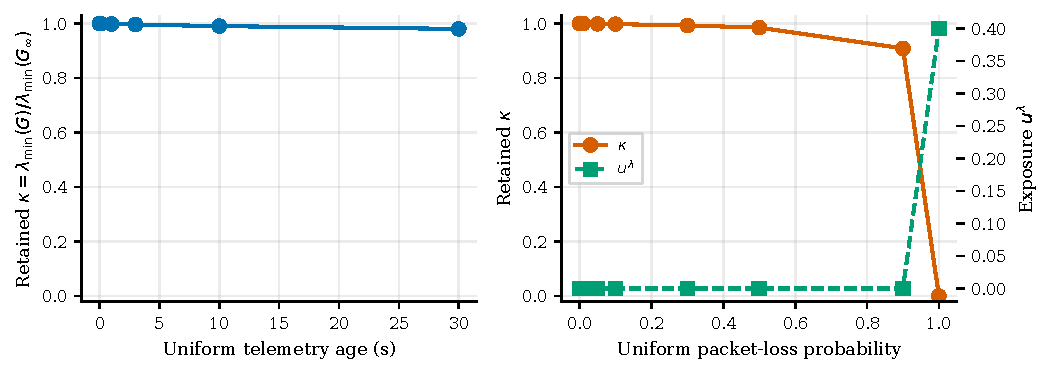
\includegraphics[width=\columnwidth]{paper1_generated/figures/fig_diagnostic_age_loss_response.pdf}
\caption{Static response to uniform age and loss. The abrupt endpoint at total loss is the observability cliff; smooth degradation away from the cliff is weak for this feeder.}
\label{fig:diagnostic-age-loss}
\end{figure}

\begin{figure}[!t]
\centering
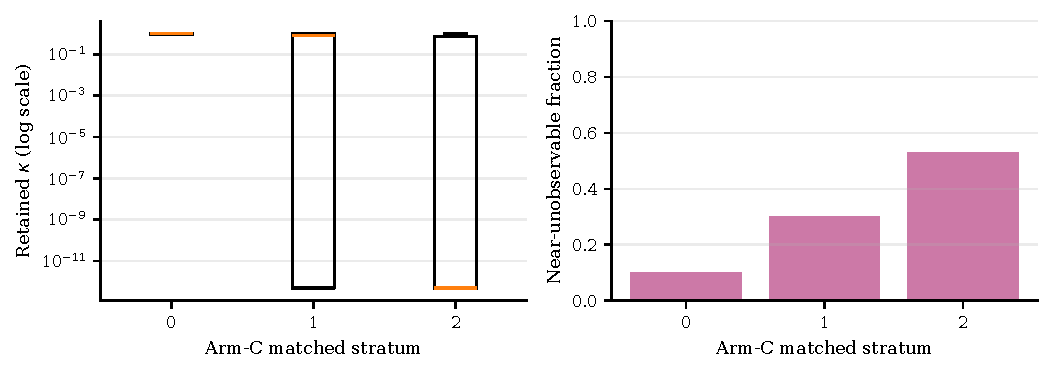
\includegraphics[width=\columnwidth]{paper1_generated/figures/fig_diagnostic_matched_identity.pdf}
\caption{Arm-C matched-count/age diagnostic. Measurement identity produces orders-of-magnitude variation in retained weak-direction information within the same trivial communication stratum.}
\label{fig:diagnostic-identity}
\end{figure}

\begin{table}[!t]
\caption{Pre-campaign Arm-C geometry diagnostic at matched received fraction and mean age. These are mechanism checks, not confirmatory detector-performance results.}
\label{tab:diagnostic-arm-c}
\centering\scriptsize
\setlength{\tabcolsep}{2.5pt}
\begin{tabular}{rrrrrr}
\toprule
Stratum & Events & $B_1$ & $B_2$ (s) & Median $\kappa$ & Near-unobs. \\
\midrule
0 & 100 & 0.822 & 0.533 & 0.993 & 10.0\% \\
1 & 100 & 0.644 & 1.067 & 0.776 & 30.0\% \\
2 & 100 & 0.467 & 1.600 & 4.9e-13 & 53.0\% \\
\bottomrule
\end{tabular}
\end{table}


\begin{figure*}[!t]
\centering
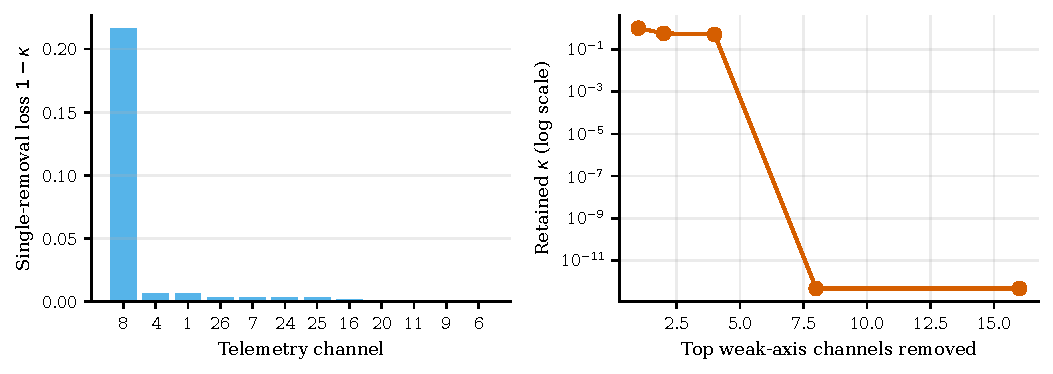
\includegraphics[width=0.88\textwidth]{paper1_generated/figures/fig_diagnostic_channel_influence.pdf}
\caption{Measurement-identity sensitivity of the weakest information direction. Left: single-channel removal loss. Right: retained information after cumulative removal of the most influential channels.}
\label{fig:diagnostic-channel-influence}
\end{figure*}

\begin{figure}[!t]
\centering
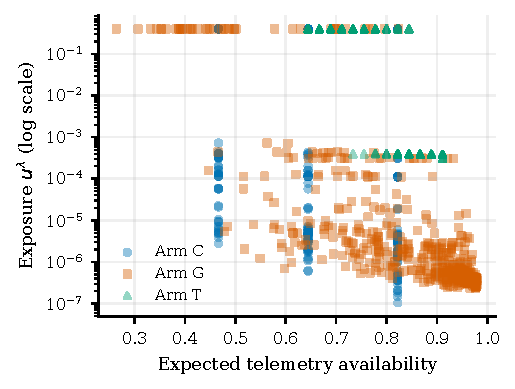
\includegraphics[width=\columnwidth]{paper1_generated/figures/fig_diagnostic_collinearity.pdf}
\caption{Static availability--exposure relationship by experimental arm. The strong but imperfect association motivates reporting collinearity and matched-pair fraction before interpreting F3.}
\label{fig:diagnostic-collinearity}
\end{figure}
%
}{%
  \begin{quote}\emph{Static diagnostic output has not yet been generated.}\end{quote}%
}
\IfFileExists{paper1_generated/latex/paper1_confirmatory_results.tex}{%
  \input{paper1_generated/latex/paper1_confirmatory_results.tex}%
}{%
  \begin{quote}\emph{The final 30-seed confirmatory campaign is pending.
  No confirmatory performance claim is made in this version.}\end{quote}%
}

% Retain the former pre-experimental layout for provenance, but do not typeset
% it in this results-ready version.

% =====================================================================
\section{Discussion}
\label{sec:discussion}

\subsection{Separability from bad-data detection and robust state estimation}
The core claim of this paper is that the proposed metric captures
something residual-based methods cannot: silent drift under communication
starvation. Two elements make that claim falsifiable. Analytically,
Proposition~\ref{prop:reduction} shows the metric reduces exactly to a
residual detector under unlimited telemetry. Under the estimator-matched
comparison, a performance difference is therefore attributable to the
communication-induced exposure term $u(t)$ rather than to a different
state estimate. The predeclared ROC-vs-bandwidth test asks
whether a difference is concentrated where residuals are least
informative and whether it vanishes toward the practically unconstrained
network level. Crucially, this argument establishes
separability from the \emph{classical} baseline only. It says nothing
about whether the information-geometric machinery is necessary, which is
why criterion F3 and the trivial controls B1--B2 of
the ablation table carry independent weight: a communication-aware
statistic as simple as the received fraction would also depart from the
residual detector under starvation. If F2 fails---no significant AUC
difference across bandwidth---the metric
is not separable from residual-based detection and we report that negative
result. If F2 passes but F3 fails, the honest conclusion is that
communication awareness matters while \emph{this} formulation does not,
and the paper should be re-scoped around the simpler statistic. If F1
fails, the phenomenon itself is not operationally significant. We commit
in advance to reporting whichever of these obtains.
\IfFileExists{paper1_generated/latex/paper1_confirmatory_discussion.tex}{%
\input{paper1_generated/latex/paper1_confirmatory_discussion.tex}%
}{The completed diagnostics establish that measurement identity can matter,
but they do not establish detector superiority. The F1--F3 verdict is
therefore withheld until the 150-cell gate passes.}

\subsection{Limitations}
\begin{itemize}
\item \emph{Simulation-only.} All evidence is from co-simulation; no
hardware or field validation is claimed. Absolute latency and rate figures
are conditioned on the fidelity of the OpenDSS and ns-3 models. Seeded
physical variation, paired trajectories, and provenance checks strengthen
internal validity but do not substitute for hardware or field evidence.
\item \emph{Assumed functional forms and constants.} The freshness
discount is no longer assumed: Lemma~\ref{lem:age} derives it from
Assumption~\ref{as:process}. This shifts the modelling burden from a free
$\tau$ to the process-noise intensity $\bQ$---physically identifiable, but
still estimated. Its misspecification now propagates through every
$\tau_i$ into \emph{both} the exposure and the residual term
(Remark~\ref{rem:ageconsistent}), so the $\bQ$ sensitivity sweep is the
most important row of Table~\ref{tab:sensitivity}. Note also that $\bQ$
now enters the \emph{estimator} through \eqref{eq:estimator}, so a
misspecified $\bQ$ degrades $\bxh$ itself and not only the metric. The combination form of $T(t)$, the exposure scalarization,
$\epsilon$, and $\omega$ remain modelling choices and are swept in
Table~\ref{tab:sensitivity}.
\item \emph{Regularization bias and saturation.} Adopting
\eqref{eq:regularized} removes the pseudo-inverse pathology
(Remark~\ref{rem:pinv}) at the cost of a bias parameter $\epsilon$ and an
exposure ceiling $u_{\max}=\omega^{2}\lmin(\bG_{\infty})/\epsilon$
(Proposition~\ref{prop:ceiling}). Under sustained blackout $T(t)$ is
therefore constant rather than continuing to fall, so the metric is a
sound \emph{detector} but not yet a graded \emph{severity} signal
(Remark~\ref{rem:saturation}).
\item \emph{Optimism under random loss --- addressed, with a caveat.}
The mean-information form understates the expected posterior covariance
\eqref{eq:jensen}; Proposition~\ref{prop:confident} supplies a
$\delta$-confident upper bound that removes the bias. The rigorous
matrix-Bernstein version can be vacuous on measurement sets of low
redundancy (Remark~\ref{rem:tightness}), in which case the tighter
direction-fixed variant must be used and its coverage reported
empirically rather than guaranteed.
\item \emph{Worst-direction scalarization.} $\lmax$ ignores the direction
in which drift actually occurs, which is the expected dominant
false-alarm mechanism (Remark~\ref{rem:direction}).
\item \emph{Linearization self-reference.} $\bG(t)$ is built from a
Jacobian evaluated at the possibly-drifted estimate
(Remark~\ref{rem:jacobian}).
\item \emph{Label validity.} Silent-drift labels come from the oracle;
their correctness depends on the oracle definition and tolerance $\gamma$.
\end{itemize}

\subsection{Threats to validity}
\begin{itemize}
\item \emph{Construct validity:} whether $d(t)>\gamma$ faithfully
operationalizes operationally significant divergence; sensitivity to
$\gamma$ is reported in Table~\ref{tab:sensitivity}. The label
deliberately does \emph{not} reference $\eta$: making residual-silence
part of the label would guarantee the classical baselines' failure by
construction (Remark~\ref{rem:circularity}).
\item \emph{Internal validity:} whether the drift-injection protocol
inadvertently makes the proposed metric's advantage artefactual---for
example by starving exactly the channels the exposure term weights
most. Independent physical and communication schedules, the predeclared
Arm C matched controls, and immutable scenario hashes are the mitigation.
\item \emph{External validity:} generalization beyond the IEEE 123-node
feeder and the specific fault data sets; additional feeders would
strengthen claims~\cite{dugan2009}.
\end{itemize}

\subsection{Open problems}
Four problems are left open, in decreasing order of how much they would
strengthen the construction.
\begin{enumerate}
\item \emph{A uniformly tight confident bound.}
Proposition~\ref{prop:confident} closes the Jensen gap, but the rigorous
matrix version is loose when $m/n$ is small
(Remark~\ref{rem:tightness}). A bound simultaneously uniform over
directions and tight at realistic redundancy---plausibly via the
intermittent-observation machinery of~\cite{sinopoli2004,schenato2007}
rather than generic matrix concentration---remains open.
\item \emph{Beyond the random-walk state model.} Lemma~\ref{lem:age}
assumes driftless Gauss--Markov dynamics. Extending it to mean-reverting
or load-driven dynamics, and to process noise correlated across phases,
would sharpen $\tau_i$ further.
\item \emph{A detectability characterization.} We provide a metric, not a
bound of the form $P_D\ge f(b,\Delta,p)$. Establishing such a bound---for
instance via a Cram\'{e}r--Rao or Chernoff argument linking excess
exposure to a minimum detectable divergence---remains open.
\item \emph{A non-saturating severity signal} for downstream control
(Remark~\ref{rem:saturation}).
\end{enumerate}

\subsection{Forward link}
The trust metric defined here is reused in subsequent thesis work as the
objective for trust-restoring sensing/communication
scheduling~\cite{bui2024,chiariotti2022} and as the trigger for
trust-triggered safe control; the saturation property of
Proposition~\ref{prop:ceiling} is a direct obstacle there and must be
addressed before that step.

% =====================================================================
\section{Conclusion}
\label{sec:conclusion}
We defined a communication-aware trust metric for distribution-grid
digital twins whose novel component is the excess silent-drift exposure
induced by finite communication, combined with a received-measurement
residual term. The metric is, by construction, an explicit function of
the communication state, and it provably reduces to the classical
$\chi^{2}$ bad-data statistic under unlimited telemetry
(Proposition~\ref{prop:reduction}, Corollary~\ref{cor:exact}), making it a
strict generalization of residual-based detection rather than a competing
heuristic. We further showed that the regularization required for
well-posedness imposes an exposure ceiling, and derived the resulting
necessary condition on the regularization level for the metric to alarm
under total starvation (Proposition~\ref{prop:ceiling}). We proposed an
evaluation against classical baselines \emph{and against trivial
communication-aware controls}, under labels defined solely by ground-truth
divergence, with three pre-registered falsification criteria covering the
existence of the phenomenon, separability from the classical baseline, and
the necessity of the information-geometric construction. Static
diagnostics confirm exact perfect-telemetry reduction and show that this
feeder's weakest information direction is highly sensitive to measurement
identity, while also revealing strong collinearity between availability
and exposure. These facts justify, but do not replace, the predeclared
confirmatory test.
\IfFileExists{paper1_generated/latex/paper1_confirmatory_conclusion.tex}{%
\input{paper1_generated/latex/paper1_confirmatory_conclusion.tex}%
}{No detector-performance conclusion is drawn before all 150 unseen-seed
cells pass the completeness and provenance gate.}
\begin{thebibliography}{99}

\footnotesize

\bibitem{tao2019} F. Tao, H. Zhang, A. Liu, and A. Y. C. Nee, ``Digital twin in industry: State-of-the-art,'' \emph{IEEE Trans. Ind. Informat.}, vol. 15, no. 4, pp. 2405--2415, Apr. 2019, doi: 10.1109/TII.2018.2873186.

\bibitem{dtgrid2026} Y. Chen, T. Tan, F. Fu, L. Ji, and J. Zuo, ``DT-Grid: A digital twin framework for real-time state awareness and operational optimization of renewable-dominated power systems,'' \emph{Electronics}, vol. 15, no. 16, Art. no. 3529, 2026, doi: 10.3390/electronics15163529.

\bibitem{moutis2021} P. Moutis and O. Alizadeh-Mousavi, ``Digital twin of distribution power transformer for real-time monitoring of medium voltage from low voltage measurements,'' \emph{IEEE Trans. Power Del.}, vol. 36, no. 4, pp. 1952--1963, Aug. 2021, doi: 10.1109/TPWRD.2020.3017355.

\bibitem{thwe2025} M. M. Thwe, A. Stefanov, V. S. Rajkumar, and P. Palensky, ``Digital twins for power systems: Review of current practices, requirements, enabling technologies, data federation and challenges,'' \emph{IEEE Access}, 2025.

\bibitem{zomerdijk2024} W. Zomerdijk, P. Palensky, T. AlSkaif, and P. P. Vergara, ``On future power system digital twins: A vision towards a standard architecture,'' \emph{Digital Twins and Applications}, vol. 1, no. 2, pp. 103--117, 2024.

\bibitem{abur2004} A. Abur and A. G\'{o}mez-Exp\'{o}sito, \emph{Power System State Estimation: Theory and Implementation}. New York, NY, USA: Marcel Dekker, 2004.

\bibitem{handschin1975} E. Handschin, F. C. Schweppe, J. Kohlas, and A. Fiechter, ``Bad data analysis for power system state estimation,'' \emph{IEEE Trans. Power App. Syst.}, vol. PAS-94, no. 2, pp. 329--337, Mar. 1975.

\bibitem{gol2014lav} M. G\"{o}l and A. Abur, ``LAV based robust state estimation for systems measured by PMUs,'' \emph{IEEE Trans. Smart Grid}, vol. 5, no. 4, pp. 1808--1814, Jul. 2014, doi: 10.1109/TSG.2014.2302213.

\bibitem{duran2023} K. Duran, M. \"{O}zdem, T. Hoang, T. Q. Duong, and B. Canberk, ``Age of twin (AoT): A new digital twin qualifier for 6G ecosystem,'' \emph{IEEE Internet Things Mag.}, vol. 6, no. 4, pp. 138--143, Dec. 2023, doi: 10.1109/IOTM.001.2300113.

\bibitem{cosandal2026} \.{I}. Cosandal and S. Ulukus, ``How far back in time a digital twin reflects the state of the physical object: Age of staleness,'' arXiv:2605.16176, May 2026. \emph{[preprint]}

\bibitem{yates2021} R. D. Yates, Y. Sun, D. R. Brown, S. K. Kaul, E. Modiano, and S. Ulukus, ``Age of information: An introduction and survey,'' \emph{IEEE J. Sel. Areas Commun.}, vol. 39, no. 5, pp. 1183--1210, May 2021, doi: 10.1109/JSAC.2021.3065072.

\bibitem{darbali2021} R. Darbali-Zamora, J. Johnson, A. Summers, C. B. Jones, C. Hansen, and C. Showalter, ``State estimation-based DER optimization for distribution voltage regulation in telemetry-sparse environments using a real-time digital twin,'' \emph{Energies}, vol. 14, no. 3, Art. no. 774, 2021, doi: 10.3390/en14030774.

\bibitem{guo2025} J. Guo, F. Chen, D. Liu, J. Weng, \emph{et al.}, ``Edge digital twin for coordinating flexible resources in distribution networks with communication constraints,'' \emph{Sci. Rep.}, vol. 15, 2025, doi: 10.1038/s41598-025-32773-6.

\bibitem{bui2024} V.-P. Bui, S. R. Pandey, P. M. de Sant Ana, B. Soret, and P. Popovski, ``Timely communication from sensors for wireless networked control in cloud-based digital twins,'' arXiv:2408.10241, Aug. 2024 (extended from IEEE ICC 2024). \emph{[preprint]}

\bibitem{molin2019} A. Molin, H. Esen, and K. H. Johansson, ``Scheduling networked state estimators based on value of information,'' \emph{Automatica}, vol. 110, Art. no. 108578, 2019.

\bibitem{voas2023} J. Voas, P. Mell, P. Laplante, and V. Piroumian, ``Security and trust considerations for digital twin technology,'' NIST Internal Report 8356, 2023, doi: 10.6028/NIST.IR.8356.

\bibitem{laplante2022} P. Laplante, ``Trusting digital twins,'' \emph{Computer}, vol. 55, no. 7, pp. 73--77, Jul. 2022.

\bibitem{jeon2024} J. Jeon and G. Theotokatos, ``A framework to assure the trustworthiness of physical model-based digital twins for marine engines,'' \emph{J. Mar. Sci. Eng.}, vol. 12, no. 4, Art. no. 595, 2024, doi: 10.3390/jmse12040595.

\bibitem{hatami2025} M. Hatami, Q. Qu, Y. Chen, J. Mohammadi, E. Blasch, and E. Ardiles-Cruz, ``ANCHOR-Grid: Authenticating smart grid digital twins using real-world anchors,'' \emph{Sensors}, vol. 25, no. 10, Art. no. 2969, 2025, doi: 10.3390/s25102969.

\bibitem{trustworthy2025} ``Toward trustworthy digital twinning: Taxonomy, analysis, and open challenges,'' \emph{Electronics}, vol. 14, no. 23, Art. no. 4732, 2025, doi: 10.3390/electronics14234732.

\bibitem{mili1985} L. Mili, T. Van Cutsem, and M. Ribbens-Pavella, ``Bad data identification methods in power system state estimation---A comparative study,'' \emph{IEEE Trans. Power App. Syst.}, vol. PAS-104, no. 11, pp. 3037--3049, Nov. 1985.

\bibitem{cheniae1996} M. G. Cheniae, L. Mili, and P. J. Rousseeuw, ``Identification of multiple interacting bad data via power system decomposition,'' \emph{IEEE Trans. Power Syst.}, vol. 11, no. 3, pp. 1555--1563, Aug. 1996.

\bibitem{gol2014three} M. G\"{o}l and A. Abur, ``A robust PMU based three-phase state estimator using modal decoupling,'' \emph{IEEE Trans. Power Syst.}, vol. 29, no. 5, pp. 2292--2299, Sep. 2014.

\bibitem{monticelli1999} A. Monticelli, \emph{State Estimation in Electric Power Systems: A Generalized Approach}. Boston, MA, USA: Springer, 1999.

\bibitem{wang2017robust} G. Wang, G. B. Giannakis, and J. Chen, ``Robust and scalable power system state estimation via composite optimization,'' \emph{IEEE Trans. Smart Grid} (also arXiv:1708.06013).

\bibitem{baran1994} M. E. Baran and A. W. Kelley, ``State estimation for real-time monitoring of distribution systems,'' \emph{IEEE Trans. Power Syst.}, vol. 9, no. 3, pp. 1601--1609, Aug. 1994.

\bibitem{singh2009} R. Singh, B. C. Pal, and R. A. Jabr, ``Choice of estimator for distribution system state estimation,'' \emph{IET Gener. Transm. Distrib.}, vol. 3, no. 7, pp. 666--678, 2009.

\bibitem{liu2011} Y. Liu, P. Ning, and M. K. Reiter, ``False data injection attacks against state estimation in electric power grids,'' \emph{ACM Trans. Inf. Syst. Secur.}, vol. 14, no. 1, Art. no. 13, May 2011, doi: 10.1145/1952982.1952995.

\bibitem{kosut2011} O. Kosut, L. Jia, R. J. Thomas, and L. Tong, ``Malicious data attacks on the smart grid,'' \emph{IEEE Trans. Smart Grid}, vol. 2, no. 4, pp. 645--658, Dec. 2011.

\bibitem{liang2017} G. Liang, J. Zhao, F. Luo, S. R. Weller, and Z. Y. Dong, ``A review of false data injection attacks against modern power systems,'' \emph{IEEE Trans. Smart Grid}, vol. 8, no. 4, pp. 1630--1638, Jul. 2017.

\bibitem{chaojun2015} G. Chaojun, P. Jirutitijaroen, and M. Motani, ``Detecting false data injection attacks in AC state estimation,'' \emph{IEEE Trans. Smart Grid}, vol. 6, no. 5, pp. 2476--2483, Sep. 2015.

\bibitem{he2017} Y. He, G. J. Mendis, and J. Wei, ``Real-time detection of false data injection attacks in smart grid: A deep learning-based intelligent mechanism,'' \emph{IEEE Trans. Smart Grid}, vol. 8, no. 5, pp. 2505--2516, Sep. 2017.

\bibitem{kaul2012} S. K. Kaul, R. D. Yates, and M. Gruteser, ``Real-time status: How often should one update?,'' in \emph{Proc. IEEE INFOCOM}, 2012, pp. 2731--2735.

\bibitem{kosta2017} A. Kosta, N. Pappas, and V. Angelakis, ``Age of information: A new concept, metric, and tool,'' \emph{Found. Trends Netw.}, vol. 12, no. 3, pp. 162--259, 2017.

\bibitem{maatouk2020} A. Maatouk, S. Kriouile, M. Assaad, and A. Ephremides, ``The age of incorrect information: A new performance metric for status updates,'' \emph{IEEE/ACM Trans. Netw.}, vol. 28, no. 5, pp. 2215--2228, Oct. 2020.

\bibitem{khan2022} L. U. Khan, Z. Han, W. Saad, E. Hossain, M. Guizani, and C. S. Hong, ``Digital twin of wireless systems: Overview, taxonomy, challenges, and opportunities,'' \emph{IEEE Commun. Surveys Tuts.}, vol. 24, no. 4, 2022.

\bibitem{mihai2022} S. Mihai \emph{et al.}, ``Digital twins: A survey on enabling technologies, challenges, trends and future prospects,'' \emph{IEEE Commun. Surveys Tuts.}, vol. 24, no. 4, pp. 2255--2291, 2022.

\bibitem{ruah2023} C. Ruah, O. Simeone, and B. Al-Hashimi, ``Digital twin-based multiple access optimization and monitoring via model-driven Bayesian learning,'' in \emph{Proc. IEEE Int. Conf. Commun. (ICC)}, 2023.

\bibitem{farag2026} H. Farag and \v{C}. Stefanovi\'{c}, ``Toward efficient deployment and synchronization in digital twins-empowered networks,'' arXiv:2604.00566, Apr. 2026. \emph{[preprint]}

\bibitem{soleymani2022} T. Soleymani, J. S. Baras, and S. Hirche, ``Value of information in feedback control: Quantification,'' \emph{IEEE Trans. Autom. Control}, vol. 67, no. 7, pp. 3730--3737, Jul. 2022.

\bibitem{chiariotti2022} F. Chiariotti, A. E. Kal\o{}r, J. Holm, B. Soret, and P. Popovski, ``Scheduling of sensor transmissions based on value of information for summary statistics,'' \emph{IEEE Netw. Lett.}, vol. 4, no. 2, pp. 92--96, Jun. 2022.

\bibitem{shi2011} L. Shi, P. Cheng, and J. Chen, ``Sensor data scheduling for optimal state estimation with communication energy constraint,'' \emph{Automatica}, vol. 47, no. 8, pp. 1693--1698, 2011.

\bibitem{sinopoli2004} B. Sinopoli, L. Schenato, M. Franceschetti, K. Poolla, M. I. Jordan, and S. S. Sastry, ``Kalman filtering with intermittent observations,'' \emph{IEEE Trans. Autom. Control}, vol. 49, no. 9, pp. 1453--1464, Sep. 2004.

\bibitem{schenato2007} L. Schenato, B. Sinopoli, M. Franceschetti, K. Poolla, and S. S. Sastry, ``Foundations of control and estimation over lossy networks,'' \emph{Proc. IEEE}, vol. 95, no. 1, pp. 163--187, Jan. 2007.

\bibitem{monticelli1985} A. Monticelli and F. F. Wu, ``Network observability: Theory,'' \emph{IEEE Trans. Power App. Syst.}, vol. PAS-104, no. 5, pp. 1042--1048, May 1985.

\bibitem{wang2018crb} G. Wang, A. S. Zamzam, G. B. Giannakis, and N. D. Sidiropoulos, ``Power system state estimation via feasible point pursuit: Algorithms and Cram\'{e}r-Rao bound,'' \emph{IEEE Trans. Signal Process.}, vol. 66, no. 6, pp. 1649--1658, Mar. 2018.

\bibitem{kersting1991} W. H. Kersting, ``Radial distribution test feeders,'' \emph{IEEE Trans. Power Syst.}, vol. 6, no. 3, pp. 975--985, Aug. 1991.

\bibitem{ieee123} IEEE PES Distribution Systems Analysis Subcommittee, ``IEEE 123-node test feeder.'' [Online]. Available: \url{https://cmte.ieee.org/pes-testfeeders/}

\bibitem{dugan2009} R. C. Dugan, W. H. Kersting, S. Carneiro, R. F. Arritt, and T. E. McDermott, ``Roadmap for the IEEE PES test feeders,'' in \emph{Proc. IEEE Power Syst. Conf. Expo. (PSCE)}, 2009, pp. 1--4.

\bibitem{palmintier2017} B. Palmintier, D. Krishnamurthy, P. Top, S. Smith, J. Daily, and J. Fuller, ``Design of the HELICS high-performance transmission-distribution-communication-market co-simulation framework,'' in \emph{Proc. Workshop Model. Simul. Cyber-Phys. Energy Syst. (MSCPES)}, 2017, doi: 10.1109/MSCPES.2017.8064542.

\bibitem{hardy2024} T. Hardy, B. Palmintier, P. Top, D. Krishnamurthy, and J. Fuller, ``HELICS: A co-simulation framework for scalable multi-domain modeling and analysis,'' \emph{IEEE Access}, vol. 12, pp. 24325--24347, 2024, doi: 10.1109/ACCESS.2024.3363615.

\bibitem{nsnam} ns-3 Project, ``ns-3 network simulator.'' [Online]. Available: \url{https://www.nsnam.org}

\bibitem{helicsns3} GMLC-TDC, ``helics-ns3: ns-3 module for integrating with a HELICS co-simulation,'' GitHub repository. [Online]. Available: \url{https://github.com/GMLC-TDC/helics-ns3}

\bibitem{delong1988} E. R. DeLong, D. M. DeLong, and D. L. Clarke-Pearson, ``Comparing the areas under two or more correlated receiver operating characteristic curves: A nonparametric approach,'' \emph{Biometrics}, vol. 44, no. 3, pp. 837--845, 1988.

\bibitem{sun2014} X. Sun and W. Xu, ``Fast implementation of DeLong's algorithm for comparing the areas under correlated receiver operating characteristic curves,'' \emph{IEEE Signal Process. Lett.}, vol. 21, no. 11, pp. 1389--1393, Nov. 2014, doi: 10.1109/LSP.2014.2337313.

\bibitem{holm1979} S. Holm, ``A simple sequentially rejective multiple test procedure,'' \emph{Scand. J. Statist.}, vol. 6, no. 2, pp. 65--70, 1979.

\bibitem{robin2011} X. Robin, N. Turck, A. Hainard, \emph{et al.}, ``pROC: An open-source package for R and S+ to analyze and compare ROC curves,'' \emph{BMC Bioinformatics}, vol. 12, Art. no. 77, 2011.

\end{thebibliography}

% =====================================================================
\end{document}
